% !TeX root = RJwrapper.tex (usually)
% LaTeX title
\title{\pkg{CovEsts}: Nonparametric Autocovariance Estimation and
Analysis}
% LaTeX author name
\author{by Adam Bilchouris and Andriy Olenko}


\maketitle

\section{Introduction}\label{introduction}

For a stationary time series \(X(j)\), \(j = 0, 1, \dots,\) the
autocovariance function is used to measure dependencies between
observations separated by a lag \(h.\) This function appears in various
theoretical results and statistical applications. For example, in the
Gaussian case, the mean function and autocovariance function describe
the time series entirely. Furthermore, the autocovariance function is
used in the estimation of parameters for an autoregressive time series
\citep[Chapter~8.1]{Brockwell1991}, model identification, and Kriging
\citep[Chapter~3.2]{Cressie1993}. It is also utilised in various
non-statistical fields such as digital signal processing, image analysis
\citep[Chapter~3.2]{Bull2021}, and quality assessment \citep{chemo2003},
just to name a few. Therefore, accurate estimation of the autocovariance
function is an important problem in numerous statistical and data
science applications.

Surprisingly, despite several other approaches in the literature, the
classical standard estimator of the autocovariance function remains the
predominant choice among practitioners. Many of them are unaware of its
limitations or of more accurate alternatives developed in the recent
literature. This is evident in statistical software, where the majority
of R and Python packages only provide a wrapper function for the
classical estimator. For example, the classical autocovariance estimator
realised by the \textbf{\texttt{stats::acf}} function in R, is used by
\CRANpkg{TSA} (\citeauthor{TSA_2022}, \citeyear{TSA_2022} and
\citeauthor{Cryer2008}, \citeyear{Cryer2008}),
\CRANpkg{astsa}~(\citeauthor{astsa_2024}, \citeyear{astsa_2024}, and
\citeauthor{Shumway2025}, \citeyear{Shumway2025}), \CRANpkg{sarima}
\citep{sarima_2024} and \CRANpkg{forecast} \citep{Hyndman2008}. The
package \CRANpkg{forecast} also contains a tapered autocovariance
estimator, \code{taperedacf()}, which is based on the results in
\cite{McMurry2010, Hyndman2015}.

The motivation for the package
\CRANpkg{CovEsts}~(\citeauthor{CovEsts_2025}, \citeyear{CovEsts_2025})
was that many nonparametric autocovariance estimators appeared only in
research papers with no R or Python code for their computation. Also, as
will be discussed in Section~\hyperref[sec:nonparametric]{2}, different
estimators have different theoretical properties, which influence when
they should be used. We have not found any packages dealing with
potential issues regarding estimation and their corrections, apart from
\CRANpkg{ncf} \citep{ncf} implementing the positive-definite adjustment
from \cite{hall1994_2}. Further, no existing packages provide a unified
interface and consistent data/output structure across various
autocovariance estimators.

Nonparametric autocovariance estimators are particularly important due
to their minimal reliance on distributional assumptions, offering
greater flexibility compared to parametric approaches. Additionally,
they are often used as a preliminary step in parametric modelling, where
a restricted set of predefined autocovariance models is fitted to a
nonparametric estimate. For example, \CRANpkg{gstat} \citep{gstat2016}
does this for the (semi-)variogram. Parametric estimation was not
included in \CRANpkg{CovEsts}, as this functionality for specific
parametric models is already provided by existing packages.

We intend this package to be used by practitioners working with time
series and spatial statistics, with applications in areas such as
finance, signal processing, and climate research. We assume basic
knowledge of \texttt{R} for using the functional interface of the
package. However, more specialised \texttt{R} knowledge may be required
for advanced inference and working with user-defined objects.

In the article, we will interchangeably use the terms random process and
time series, where the former is for samples at arbitrary time
locations, and the latter is used when sampled values are on a uniform
sampling grid.

The paper is structured as follows.
Section~\hyperref[sec:nonparametric]{2} introduces the nonparametric
autocovariance estimators and some general approaches for modifying
autocovariance estimators. It discusses the theoretical properties of
the estimators and the drawbacks one should be aware of.
Section~\hyperref[sec:overview]{3} presents the structure of the package
and selected main functions. Section~\hyperref[sec:examples]{4} provides
applications to three data examples: a simulated Gaussian process,
yearly sunspot counts, and unemployment data, sourced from the US Bureau
of Labor Statistics. Example 4 empirically studies the computational
complexity of the estimators by comparing their memory and time usage.

\section{Nonparametric estimators of autocovariance
functions}\label{sec:nonparametric}

There are several nonparametric autocovariance function estimators in
the literature, see the reviews in \citet[Chapter~2.4]{Cressie1993},
\citet{hall1994_2}, \citet{cuevas2013study}, \citet{Durre2015} and
\citet{Bilchouris_Olenko_2025}. This section briefly introduces the
estimators that were implemented in the package and mentions some of the
theoretical drawbacks to deal with when applying them.

For a weakly stationary real-valued time series \(X(j)\),
\(j = 1, 2, \dots ,\) the autocovariance function is defined as
\[\text{C}(h) \coloneq \text{E}\left[\left(X(j) - \overline{X}\right)\left(X(j + h) - \overline{X}\right)\right].\]
and the corresponding autocorrelation at lag \(h\) is
\(\rho(h):=C(h)/C(0).\)

Another related function used in the analysis of dependencies is the
semivariogram. It uses the second-order moments of increments,
\[\gamma(h) := \frac{1}{2} \text{Var}\left[X(j) - X(j + h) \right]  ,\]
The package \CRANpkg{CovEsts} mainly focuses on estimating \(C(\cdot)\)
as, under the assumption of weak stationarity, the semivariogram can be
determined using the autocovariance function through the following
relation \begin{equation}
 \label{eqn:variogram}
    \gamma(h) = C(0) - C(h).
\end{equation} This relation is not necessarily true when considering
the estimated functions or if the semivariogram is unbounded
(\citeauthor{Chils2012}, \citeyear{Chils2012} and
\citeauthor{Bilchouris_Olenko_2025}, \citeyear{Bilchouris_Olenko_2025}).

Another function used in time series analysis is the partial
autocorrelation function, \(\phi_{h,h}.\) Unlike the autocorrelation
function, it measures the dependencies between observations \(X(t)\) and
\(X(t+h)\) after removing the effects of the intermediary lags. The
partial autocorrelation function at lag \(h\) can be computed using the
Durbin-Levinson algorithm \citep{Durbin1960} \begin{equation}
 \label{eq:durbin}
    \phi_{h, h} \coloneq \frac{\rho(h) - \sum_{k=1}^{h-1} \phi_{h - 1, k} \rho(h - j)}{1 - \sum_{k=1}^{h-1} \phi_{h - 1, k} \rho(k)}
\end{equation} where
\(\phi_{h, k} := \phi_{h - 1, k} - \phi_{h, h} \phi_{h - 1, h - k}\) for
\(k = 1, 2, \dots, h - 1,\) and \(\phi_{1, 1} := \rho(1)\). Unlike the
autocorrelation function, there is no zero lag for the partial
autocorrelation function. In \textbf{stats::pacf}, the formula
(\ref{eq:durbin}) uses the classical autocorrelation estimator, but any
autocorrelation estimate can be supplied in the package
\CRANpkg{CovEsts}.

\subsection{Standard estimators}\label{standard-estimators}

The first two estimators implemented in \CRANpkg{CovEsts} are well-known
and the most widely used. They differ only by the normalising constants:
\begin{equation}
 \label{eq:std_est}
\widehat{C}^{*}(h) \coloneq \frac{1}{N-h} \sum_{j=1}^{N - h} \left(X(j) - \overline{X}\right) \left(X(j+h) - \overline{X}\right)
\end{equation} and \begin{equation}
 \label{eq:std_est_pd}
\widehat{C}^{**}(h) \coloneq \frac{1}{N} \sum_{j=1}^{N - h} \left(X(j) - \overline{X}\right) \left(X(j+h) - \overline{X}\right) ,
\end{equation} where \(X(j)\) represents values of an observed time
series, \(\overline{X}\) is the sample mean of the time series, \(N\) is
the length of the observation period and \(0 \leq h \leq N-1\) is the
lag for which the autocovariance function is estimated at
\citep[Section~3.17]{Yaglom1987}. These estimators are typically used
for equally sampled values at integer time moments or those with a
constant time difference.

Even for these classical estimators, there are several issues that are
not expected when applying autocovariance functions in theoretical
statistical inference. The first estimator \eqref{eq:std_est} is
unbiased if the mean \(\text{E}[X(j)]\) is known and used instead of
\(\overline{X},\) but is biased otherwise \citep{Brockwell2016}. This
estimator is not positive-definite. The estimator~\eqref{eq:std_est_pd}
is biased but is positive-definite. This means that the second estimator
gives a true autocovariance function, whilst the first only gives an
estimate of a function similar to an autocovariance function.

Another, less-known drawback is that when considering the sum over all
lags for the estimated autocorrelations in \eqref{eq:std_est_pd}, the
sum is always equal to \(-1/2\), regardless of the sampled values, see
\cite{Hassani2009}, \citet{Hassani2012} and
\cite{Bilchouris_Olenko_2025}. This causes a problem, especially when
considering estimation over long time intervals or modelling long-range
dependence, as the sum of estimated autocorrelation values is always
equal to \(-1/2\). Even though the estimators have desirable theoretical
properties for a fixed \(h,\) when \(N  \rightarrow \infty ,\) the
constant sum necessitates substantial departure of the estimates from
the true autocovariance values if a large range of \(h\) is considered
for a fixed \(N.\)

\subsection{Kernel regression
estimators}\label{kernel-regression-estimators}

The next estimator, proposed in \citet{hall1994} and \citet{hall1994_2},
applies the kernel regression of pairwise autocovariances to estimate
the autocovariance function, \begin{equation}
 \label{eq:hall_est}
\widehat{C}_{H}(t) \coloneq \frac{\displaystyle \sum_{i=1}^{N} \sum_{j=1}^{N}  \check{X}_{ij} K\left( \left(t - \left(t_{i} - t_{j}\right)\right) / b \right) }{\displaystyle \sum_{i=1}^{N} \sum_{j=1}^{N}  K\left( \left(t - \left(t_{i} - t_{j}\right)\right) / b \right) },
\end{equation} where \(t, t_{i}, t_{j} \in \mathbb{R},\)
\(\check{X}_{ij} \coloneq \left(X(t_{i}) - \overline{X}\right) \left(X(t_{j}) - \overline{X}\right)\),
\(i, j = 1, \dots, N,\) \(K(\cdot)\) is a kernel which has the
properties of a symmetric probability density and \(b > 0\) is some
bandwidth. A variant of this estimator, proposed in \cite{hall1994_2},
brings the initial estimator down to zero linearly between time moments
\(T_{1} > 0\) and \(T_{2} > T_{1},\) \begin{equation}
 \label{eq:hall_trunc}
    \widehat{C}_{1}(t): =
    \begin{cases}
        \widehat{C}_{H}(t), & 0 \leq t \leq T_{1} \\
        \widehat{C}_{H}\left(T_{1}\right) \left(T_{2} - t\right) \left(T_{2} - T_{1}\right)^{-1}, &  T_{1} < t \leq T_{2} \\
        0 , & t > T_{2} .
    \end{cases}
\end{equation} This estimator cannot be used for long-memory time series
as it vanishes at \(T_{2} ,\) but is a better choice when estimating a
short-range dependent autocovariance function, as the estimate will go
to zero. Unlike estimators~\eqref{eq:std_est} and \eqref{eq:std_est_pd},
these estimators can be applied for arbitrary observation grids and
lags.

The estimators given by \eqref{eq:hall_est} and \eqref{eq:hall_trunc}
are not necessarily positive-definite, and thus not valid autocovariance
functions. Two corrections to make them positive-definite were proposed
in \citet{hall1994} and \citet{hall1994_2}.

\begin{itemize}
\item
  \label{make_pos_def_1} The first correction method computes the
  Fourier transform of \eqref{eq:hall_est} to obtain the corresponding
  spectral density. Then, it makes any negative values in the spectral
  density equal to zero, and performs the inverse Fourier transform to
  obtain a positive-definite estimate of the autocovariance function.
  The modification of the spectral density that corresponds to
  \(\widehat{C}_{H}(\cdot)\) can be expressed as
  \(\widetilde{\mathcal{F}}(\theta) := \max(\widehat{\mathcal{F}}(\theta), 0)\)
  for every frequency \(\theta ,\) where
  \(\widehat{\mathcal{F}}( \cdot )\) and
  \(\widetilde{\mathcal{F}} ( \cdot )\) denote the original and modified
  spectral densities.
\item
  \label{make_pos_def_2} The second correction method considers
  manipulating the Fourier transform again. However, it finds the
  smallest frequency corresponding to a negative value in the spectral
  density. Then, it sets all values in the spectrum to zero whose
  corresponding frequencies are larger than the smallest frequency.
  Then, the inverse Fourier transform is taken. The process of selecting
  the frequency and modifying the spectrum is as follows. Let
  \(\widehat{\theta} := \inf \left\{ \theta > 0 : \widehat{\mathcal{F}} \left( \theta \right) < 0 \right\}.\)
  Then the spectral density is modified as follows,
  \(\widetilde{\mathcal{F}}(\theta) := \widehat{\mathcal{F}}(
  \theta)\bm{1}\left(\theta < \widehat{\theta}\right),\) where
  \(\bm{1}(A)\) is the indicator function of a set \(A.\) The drawback
  is that this correction can fail to produce a meaningful result if
  \(\widehat{\theta}\) is a small frequency, as the modified estimator
  of the autocovariance function consists of a sum of only a few
  cosines. Both of these correction methods can be applied to any
  estimator of the autocovariance function, one is not restricted to
  just estimators~\eqref{eq:hall_est} and \eqref{eq:hall_trunc}.
\end{itemize}

\subsection{Tapered estimators}\label{tapered-estimators}

The following estimator, proposed in \cite{Dahlhaus1987}, takes the edge
effect into account. The edge effect reflects the situation that points
closer to the boundaries of an observation region can have neighbouring
observations that are outside of the study region. Thus, some
dependencies may not be properly reflected, which can introduce bias. To
deal with this, the estimator assigns weights for each location
depending on how close it is to the boundary, where lower weights are
given to locations closer to the boundaries: \begin{equation}
 \label{eq:tapered_est}
        \widehat{C}^{a}_{N}(h) \coloneq \frac{\displaystyle \sum_{j = 1}^{N - h} \left( X(j) - \overline{X}\right) \left( X(j + h) - \overline{X} \right) a\left( (j - 1/2)/N; \rho \right) \; a \left( (j + h - 1/2)/N; \rho \right) }
        {\displaystyle H_{2, N}(0) },
\end{equation} where the normalising factor is
\[H_{2, N}(0) := \sum_{s=1}^{N} a ( (s - 1/2)/N; \rho )^{2} ,\]
\(a(\cdot; \cdot)\) is a taper function on the interval \([0, 1]\) with
the smoothness parameter \(\rho \in (0, 1],\) \[a(u; \rho) := 
\begin{cases}
        w(2u/\rho) ,& 0 \leq u < \frac{1}{2}\rho, \\
        1 ,& \frac{1}{2} \rho \leq u \leq \frac{1}{2}, \\
        a(1-u; \rho) ,& \frac{1}{2} < u \leq 1,
\end{cases}\] and \(w(\cdot)\) is a continuous nondecreasing function on
\([0, 1]\) with \(w(0)=0\) and \(w(1)=1.\) We will refer to \(w(\cdot)\)
as a window function. The estimator~\eqref{eq:tapered_est} is
positive-definite and biased, but the bias is negligible asymptotically.
This estimator is applied to observations on an integer grid.

\subsection{Splines estimators}\label{splines-estimators}

Unlike the other estimators, the following estimator does not use
observations directly. It is based on an approximation of
\(\widehat{C}(\cdot)\) by completely monotone basis functions proposed
in \cite{Choi2013}\\
\begin{equation}
 \label{eq:splines_est}
    \widehat{C}^{B}(h) \coloneq \sum_{j=1}^{m + p} \beta_{j} f_{j}^{(p - 1)} \left(h^{2}\right) ,
\end{equation} where \(\beta_{j} \geq 0\),
\(f_{j}^{(l)} (x) \coloneq \int_{0}^{1} (m + 1) t^{x} B_{j + 1}^{(l)} (t) \text{d} t,\)
\(B_{j}^{(l)}(\cdot)\) is the \(j^{\text{th}}\) B-spline of order \(l\)
and \(j = 1, 2, \dots , m + p\). The constants \(\beta_{j}\) are chosen
via weighted least squares, where the objective function is
\[\sum_{i = 1}^{L} w_{i} \left( \widehat{C}(h_{i}) - \sum_{j=1}^{m + p} \beta_{j} f_{j}^{(p - 1)} \left(h_{i}^{2}\right) \right)^{2} ,\]
\(\widehat{C}(\cdot)\) is an autocovariance function estimator,
\(\{ h_{1} , \dots , h_{L} \}\) is a set of lags and
\(\{ w_{1}, \dots , w_{L} \}\) is a set of weights. \cite{Choi2013} uses
\eqref{eq:std_est} as \(\widehat{C}(\cdot)\), however, one can use any
autocovariance estimator. For the choice of weights
\(w_{i} = \left(N-h_{i}\right) / \left(1 - \widehat{C}(h_{i})\right)^{2}\)
was proposed in \cite{Cressie1985}.

This estimator can calculate the estimated autocovariance at an
arbitrary lag once the fitting process is done. However, the lags used
during the fitting process should be chosen such that they are the same
as in \(\widehat{C}(\cdot).\) As estimator~\eqref{eq:splines_est} is
constructed using completely monotone basis functions, and
\(\beta_{j} \geq 0,\) it is nonnegative. This estimator is a
positive-definite function. Further, it is also bounded from below by
zero, meaning this estimator cannot be used when the autocovariance is
below zero, and due to the monotonicity, it cannot be used if
cyclicality is present.

\subsection{Kernel correction
estimators}\label{kernel-correction-estimators}

The next estimator is simply a modification of any estimator. It was
proposed to remove estimation \dfn{wave} artefacts
\citep[Section~3.17]{Yaglom1987}. The waves are present in various
estimated autocovariance functions and are more prominent as the
estimation lag increases, as fewer points are available to compute the
autocovariance function. This estimator also helps to reduce constant
summation effects, which were discussed earlier for
estimators~\eqref{eq:std_est} and \eqref{eq:std_est_pd}. It is defined
as \begin{equation}
 \label{eqn:kernel_correction}
    \widehat{C}_{T}^{(a)}(h) \coloneq a_{T}(h) \widehat{C}(h) ,
\end{equation} where \(a_{T}(\cdot)\) is a kernel function, which
approaches zero as \(\left| h \right|\) increases and
\(\widehat{C}(\cdot)\) is any autocovariance estimator
\citep[Section~3.17]{Yaglom1987}. Typically,
\(a_{T}(h) \coloneq a(h / N_{T})\), where \(N_{T}\) is some constant,
usually 10\% of the number of observations. If \(a_{T}(\cdot)\) is
chosen as positive-definite and \(\widehat{C}(\cdot)\) is
positive-definite, then \(\widehat{C}_{T}^{(a)}\) will also be
positive-definite.

A combination of \eqref{eq:std_est_pd} and \eqref{eqn:kernel_correction}
can also be used to reduce the waves in the estimate and guarantee a
finite range of dependencies: \begin{equation}
 \label{eqn:kernel_correction_std_pd}
    \widehat{C}_{T}^{**}(h) = a_{T}(h) \widehat{C}^{**}(h) .
\end{equation}

\subsection{Linear shrinking}\label{linear-shrinking}

A linear shrinkage correction method, introduced by \citet{Devlin1975},
adjusts the estimated autocorrelation matrix \(\bm{R}\) through the
following transformation \begin{equation}
 \label{eqn:linear_shrinking}
    \widetilde{\bm{R}} \coloneq \lambda \bm{R} + (1 - \lambda)\bm{I}_{p} ,
\end{equation} where \(\widetilde{\bm{R}}\) is the shrunken
autocorrelation matrix, \(\lambda \in [0, 1]\) is the shrinking
coefficient and \(\bm{I}_{p}\) is the \(p \times p\) identity matrix,
often called the shrinkage target \citep{Rousseeuw1993}. \(\lambda\) is
chosen as the maximal value for which \(\widetilde{\bm{R}}\) remains
positive-definite.

\subsection{Block bootstrap}\label{block-bootstrap}

The moving block bootstrap, independently developed by \cite{Kunsch1989}
and \cite{Liu1992}, allows for the resampling of time series data with
dependencies without relying on any parametric
assumptions~\citep[Chapter~2.5]{Lahiri2003}. For a time series
\(X(1), \dots , X(n)\), first, construct \(n - \ell + 1\) blocks of
length \(\ell,\)
\(\mathcal{B}_{i} = \left( X(i), \dots , X(i + \ell - 1) \right),\) for
\(i = 1, \dots , n - \ell + 1.\) Then, the blocks are sampled in the
following way. Let \(I_{1}, \dots, I_{k}\) be \(k\) independent and
identically sampled values, from the discrete uniform distribution on
\(\left\{ 1,\dots, n - \ell + 1 \right\},\) which are the block indices,
that is \(\mathcal{B}_{I_{i}}.\) To construct a bootstrapped time
series, join the randomly sampled blocks
\(\mathcal{B}_{I_{1}}^{*}, \dots, \mathcal{B}_{I_{k}}^{*},\) resulting
in the time series \(X^{*}(1), \dots, X^{*}(k\ell),\) where \(*\)
denotes the sampled versions of the blocks and time series
\cite[Chapter~2.5]{Lahiri2003}. If \(k\ell>n,\) the moving block sampled
time series is truncated at \(n.\)

The moving block bootstrap suffers from a boundary effect, where lesser
weights are given to observations at the beginning and end of the
sampled time series \citep[Chapter~2.7]{Lahiri2003}. A modified method
to construct bootstrap samples is the circular bootstrap, proposed by
\cite{Politis1992}, which addresses this issue. Instead of the time
series \(X(1) , \dots , X(n)\) being observed on the line, it is
considered to be observed on the circle. This results in the observation
\(X(n + k)\) being the same as \(X(k)\) for \(k = 1, \dots , n.\) For
\(i = 1, \dots , n ,\) blocks are constructed in a similar, but circular
fashion. For example, the block
\(\mathcal{B}_{n - \ell + 2} = \left(X(n - \ell + 2) , \dots , X(n), X(n + 1) \right)\)
is the same as \(\left(X(n - \ell + 2) , \dots , X(n), X(1) \right) .\)
The procedure to construct a circular bootstrap time series is the same
as for the moving block bootstrap. However, the block indices are
instead sampled from \(\{1, \dots , n\}\).

The block length parameter choice is flexible, although some guidelines
exist, see \cite{Hall1995}, \cite{Politis2004} and \cite{Arteche2024}.
For example, a block length \(\ell \sim C n^{1/k}, k = 3, 4, 5,\) is
recommended in \citep{Hall1995}. For a time series with long memory, the
block bootstrap may give inconsistent results, see \cite{Lahiri1993}. In
such cases, a larger block size should be chosen to capture the
dependency structure.

In the context of autocovariance estimation in this paper, first, a
block bootstrap method is used to sample multiple time series. Then, a
specified autocovariance estimation method is applied to compute the
estimated autocovariance for each sampled time series. The bootstrap
estimate is the average of all individual estimators, and the
corresponding bootstrap confidence region is constructed from the
bootstrap confidence intervals at each lag \(t\) of the considered
autocovariance estimate.

Table~\ref{tab:tab_summary} summarises some properties of the estimators
presented in this section, including their input requirements,
assumptions of grid regularity, positive-definiteness, computational
efficiency, suitability for long-memory processes, and disadvantages
that applied users should be aware of.

Additional theoretical results and formulas will be introduced later
when needed.

\setlength{\tabcolsep}{3pt}

\centering

\protect\phantomsection\label{tab:tab_summary}
\begin{longtable}[]{@{}lcccccc@{}}
\caption{Summary of selected properties of the
estimators}\tabularnewline
\toprule\noalign{}
\endfirsthead
\endhead
\bottomrule\noalign{}
\endlastfoot
{Estimator} & {Input} & {Grid} & {P.d.} & & & \\
efficiency & & & & & & \\
long memory & {Disadvantages} & & & & & \\
Standard~(3) & Data & Regular & No & Fast & No & \\
summation & & & & & & \\
Standard~(4) & Data & Regular & Yes & Fast & No & \\
summation & & & & & & \\
Hall's~(5) & Data & Both & No & Slow/unstable & Yes & \\
time series & & & & & & \\
Hall's Truncated~(6) & Data & Both & No & Slow/unstable & No & \\
time series & & & & & & \\
Hall's Correction~(i) & Cov.est. & Regular & Yes & Fast & No &
\makecell{Inflates est.variance} \\
Hall's Correction~(ii) & Cov.est. & Regular & Yes & Fast & No & \\
to few cosines & & & & & & \\
Tapered~(7) & Data & Regular & Yes & Fast & Yes & \\
cause bias & & & & & & \\
Splines~(8) & & & & & & \\
Cov.est. & From Cov.est. & Yes & Slow/unstable & No & & \\
nonnegative & & & & & & \\
Kernel Correction~(9) & Cov.est. & Regular & No & Fast & No & \\
memory nature & & & & & & \\
Kernel Correction~(10) & Cov.est. & Regular & No & Fast & No & \\
memory nature & & & & & & \\
Shrinkage Correction~(11) & Data & Regular & No & From Cov.est. & & \\
dependent & & & & & & \\
wrong target & & & & & & \\
& & & & & & \\
bootstrap average & Data & From Cov.est. & No & From Cov.est. & From
Cov.est. & \\
boundary effect & & & & & & \\
& & & & & & \\
average & Data & From Cov.est. & No & From Cov.est. & From Cov.est. & \\
information, & & & & & & \\
Edge jumps & & & & & & \\
\end{longtable}

\section{Package structure and function overview}\label{sec:overview}

This section provides a high-level overview of the package, including
the types of functions and their relations, function structures, and the
parameters of selected functions.

\subsection{Package interface and S3 objects
overview}\label{package-interface-and-s3-objects-overview}

The package \CRANpkg{CovEsts} consists of several functions to compute
the autocovariance estimators discussed in the previous section. For the
\CRANpkg{CovEsts} package, we deliberately aimed to keep the number of
package dependencies minimal, so it only uses packages that come with
base R, \pkg{stats} for \texttt{acf}, \texttt{optim} and \texttt{fft},
\pkg{graphics} for \texttt{legend}, \texttt{lines} and \texttt{polygon},
and \pkg{parallel} for \texttt{parLapply}, \texttt{makePSOCKcluster},
\texttt{clusterExport} and \texttt{stopCluster}. This was done to make
the package self-contained.

Figure~\ref{fig:functions_group} groups the main functions depending on
their functionality and relations to the autocovariance estimation
functions. The main group, \emph{Autocovariance Estimators}, consists of
the autocovariance function estimators discussed in
Section~\hyperref[sec:nonparametric]{2}, whilst the remaining groups are
used for intermediary and complementary calculations, except those that
compare autocovariance estimates. Note that this figure does not include
all functions in the package. In particular, non-user-facing functions
are omitted.

In the main group, there are nine functions that estimate the
autocovariance function or its modifications. As the parameters are
often shared or similar between the estimator functions, to avoid
repetition, only one set of parameters is shown in
Table~\ref{tab:truncated_est_params}. As can be seen from the table, the
functions are vectorised.

\begin{figure}[htb!]
\centering
\begin{minipage}[t]{0.45\linewidth}
\centering
\end{minipage}
\hfill
\begin{minipage}[t]{0.45\linewidth}
\begin{tikzpicture}
    \tikzstyle{block} = {draw, rectangle, align=center, minimum width=2cm, minimum height=1cm}
    \tikzstyle{line} = [draw, -latex']

    % Center
    \node [block,align=center]  (cov_ests) {\uline{Autocovariance Estimators}\\
        {\ttfamily standard\_est}\\
        {\ttfamily adjusted\_est}\\
        {\ttfamily truncated\_est}\\
        {\ttfamily tapered\_est}\\
        {\ttfamily splines\_est}\\
        {\ttfamily kernel\_est}\\
        {\ttfamily corrected\_est}\\
        {\ttfamily to\_vario}\\
        {\ttfamily to\_pacf}\\
        {\ttfamily block\_bootstrap}};

    % LEFT (slightly up)
    \node [block, align=center, left = 1.2cm of cov_ests, yshift=1.3cm] (general) {\uline{General Functions}\\
        {\ttfamily dct\_1d}\\
        {\ttfamily idct\_1d}\\
        {\ttfamily make\_pd}\\
        {\ttfamily nearest\_pd}\\
        {\ttfamily shrinking}};

    % LEFT BELOW (also shifted up)

      \node [block, align=center, below = 0.4cm of general] (kernels) {\uline{\shortstack{Kernel and Window\\Functions}}\\
        {\ttfamily kernel\_ec}\\
        {\ttfamily kernel\_symm\_ec}\\
        {\ttfamily window\_ec}\\
        {\ttfamily window\_symm\_ec}};

    % RIGHT
  \node [block, align=center, right = 1.2cm  of cov_ests, yshift=1.1cm] (metrics) {\uline{Metric Functions}\\
        {\ttfamily area\_between}\\
        {\ttfamily max\_distance}\\ 
        {\ttfamily spectral\_norm}\\
        {\ttfamily check\_pd}\\
        {\ttfamily hilbert\_schmidt}\\
        {\ttfamily mse}};

       % RIGHT BELOW
 \node [block, align=center,  below = 0.4cm of metrics] (helpers) {\uline{Helper Functions}\\
        {\ttfamily taper}\\
        {\ttfamily normalise\_acf}\\
        {\ttfamily bootstrap\_sample}\\
        {\ttfamily starting\_locs}};

    % Arrows (anchored to left side of center block)
   \draw [<-] ($(cov_ests.north west)!0.43!(cov_ests.south west)$) -- (general.east);
\draw [<-] ($(cov_ests.north west)!0.7!(cov_ests.south west)$) -- (kernels.east);
 \draw [->] ($(cov_ests.north east)!0.43!(cov_ests.south east)$)(cov_ests) -- (metrics.west);
    \draw [<-] ($(cov_ests.north east)!0.7!(cov_ests.south east)$) -- (helpers.west);

\end{tikzpicture}
\end{minipage}
\caption{Types and links between main package
functions.}\label{fig:functions_group}
\end{figure}

\centering

\protect\phantomsection\label{tab:truncated_est_params}
\begin{longtable}[]{@{}
  >{\raggedright\arraybackslash}p{(\linewidth - 2\tabcolsep) * \real{0.0000}}
  >{\raggedright\arraybackslash}p{(\linewidth - 2\tabcolsep) * \real{0.7700}}@{}}
\caption{Example of parameters for
\protect\texttt{truncated\_est}}\tabularnewline
\toprule\noalign{}
Parameter & \begin{minipage}[b]{\linewidth}\raggedright
Explanation
\end{minipage} \\
\midrule\noalign{}
\endfirsthead
\toprule\noalign{}
Parameter & \begin{minipage}[b]{\linewidth}\raggedright
Explanation
\end{minipage} \\
\midrule\noalign{}
\endhead
\bottomrule\noalign{}
\endlastfoot
\texttt{X} & A vector representing observed values of the time
series. \\
\texttt{x} & A vector of lags. \\
\texttt{t} & The arguments at which the autocovariance function is
calculated. \\
\texttt{T1} & The first truncation point, \(T_{1} > 0.\) \\
\texttt{T2} & The second truncation point, \(T_{2} > T_{1} > 0.\) \\
\texttt{b} & Bandwidth parameter, greater than 0. \\
\texttt{kernel\_name} & The name of the symmetric kernel function to be
used. Possible values are: gaussian, wave, rational\_quadratic, and
bessel\_j. Alternatively, a custom kernel function can be provided. \\
\texttt{kernel\_params} & A vector of parameters of the kernel
function. \\
\texttt{custom\_kernel} & If a custom kernel is to be used or not.
Defaults to \texttt{FALSE}. \\
\texttt{pd} & Whether a positive-definite estimate should be used.
Defaults to \texttt{TRUE}. \\
\texttt{type} & Compute either the `autocovariance' or
`autocorrelation'. Defaults to `autocovariance'. \\
\texttt{meanX} & The average value of \texttt{X}. Defaults to
\texttt{mean(X)}. \\
\texttt{parallel} & Whether or not the computations should be done in
parallel or not. Defaults to \texttt{FALSE}. \\
\texttt{ncores} & The number of cores to be used in the parallel
computations. Defaults to the number cores - 1 (threads if
hyperthreading is available), calculated from
\texttt{parallel::detectCores()\ -\ 1}. \\
\texttt{cl\_export} & A vector of any additional functions or variables
to export for parallel computations. This may be required if
\code{estimator} is not within the package. Defaults to
\texttt{NULL}. \\
\texttt{cl} & An optional cluster object created by
\code{parallel::makeCluster}. Defaults to \code{NULL}, which creates a
temporary PSOCK cluster. \\
Return & A CovEsts S3 object containing the truncated kernel regression
estimates, the lags, the estimated type and the estimator used. \\
\end{longtable}

The estimator functions are called through a single function, accepting
a time series as the first argument, and additional arguments depending
on the estimation method. As the first argument is the time series, the
pipe operator \code{|>} can be used for all estimators, for example,
\code{X\,|>\,truncated\_est(other arguments)}. All autocovariance
estimator functions return a \textbf{\texttt{CovEsts}} S3 object. These
S3 objects are lists containing four elements,

\begin{itemize}
\item
  \code{acf}: the estimated autocovariance/autocorrelation/partial
  autocorrelation values,
\item
  \code{lags}: the lag indices used to compute the estimates on,
\item
  \code{est\_type}: the type of estimate, namely `autocorrelation',
  `autocovariance' or `partial',
\item
  \code{est\_used}: the estimator function used.
\end{itemize}

In addition to the \textbf{\texttt{CovEsts}} S3 objects, there are also
the \textbf{\texttt{VarioEsts}} and \textbf{\texttt{BootEsts}} S3
objects for variograms computed using \texttt{to\_vario} and for block
bootstrap estimates. The \textbf{\texttt{VarioEsts}} object has the
following elements,

\begin{itemize}
\item
  \code{acf}: the estimated variogram values,
\item
  \code{lags}: the lag indices used to compute the estimates on,
\item
  \code{est\_type}: `to\_vario'.
\end{itemize}

The \textbf{\texttt{BootEsts}} has several more elements,

\begin{itemize}
\item
  \code{avg\_acf}: the average bootstrap autocovariance/autocorrelation
  function estimate,
\item
  \code{lags}: the lag indices used to compute the estimates on,
\item
  \code{acf\_orig}: the nonbootstrapped autocovariance/autocorrelation
  estimate,
\item
  \code{acf\_mat}: a matrix of all of the bootstrap estimates,
\item
  \code{conf\_lower}: the lower bounds for the estimated pointwise
  confidence interval,
\item
  \code{conf\_upper}: the upper bounds for the estimated pointwise
  confidence interval,
\item
  \code{est\_type}: the type of estimate, namely `autocorrelation',
  `autocovariance',
\item
  \code{est\_used}: the estimator function used,
\item
  \code{boot\_type} is either `moving' or `circular' depending on the
  type of block bootstrap used,
\item
  \code{alpha} is the \(\alpha\) value used to compute the confidence
  intervals.
\end{itemize}

All these S3 objects have \texttt{print}, \texttt{plot} and
\texttt{lines} methods. The \texttt{lines} method allows easy comparison
between the obtained estimates. For \textbf{\texttt{CovEsts}} and
\textbf{\texttt{VarioEsts}} it overlays a line directly on the plot. The
\code{lines} method for \textbf{\texttt{BootEsts}} plots a single
averaged estimate across all bootstrap samples, rather than displaying
the individual estimates corresponding to each bootstrap sample.

S3 objects were chosen over S4 and R6 due to their simplicity, both
internally and in terms of user-facing flexibility. Namely, they allow
plotting and printing the obtained estimates as ordinary \texttt{R}
objects, without requiring inspection of the underlying list structure.
This is particularly useful when plotting multiple results together,
enabling an easy comparison. Further, if a user wishes to extract the
estimated values or any other elements, this can be done
straightforwardly.

\subsection{Main estimators}\label{main-estimators}

To compute the standard estimator~\eqref{eq:std_est}, one uses the
function

\begin{verbatim}
standard_est(X, pd = TRUE, maxLag = length(X) - 1, x = 0:length(X),
        type = c("autocovariance", "autocorrelation"), meanX = mean(X)) ,
\end{verbatim}

where \texttt{maxLag} \(\leq N - 1\) is the maximum lag for which the
estimated autocovariance function is computed and \texttt{x} are the
indices for which the time series was observed on. To obtain the
estimate~\eqref{eq:std_est_pd}, \texttt{pd\ =\ TRUE} should be used
instead. As can be seen, this function assumes the basic case of equally
spaced observations on a consecutive grid of points, such as the
integers or those with a constant difference of the observation period.
This function, along with all other estimator functions with the
"\code{\_est}" suffix, returns a \textbf{\texttt{CovEsts}} S3 object.

To provide examples of other function calls, we consider
estimators~\eqref{eq:hall_est} and \eqref{eq:hall_trunc} that can be
computed through the commands

\begin{verbatim}
adjusted_est(X, x, t, b,
        kernel_name = c("gaussian", "wave", "rational_quadratic", "bessel_j"),
        kernel_params=c(), pd = TRUE, type = c("autocovariance", "autocorrelation"),
        meanX = mean(X), custom_kernel = FALSE, parallel = FALSE,
        ncores = parallel::detectCores() - 1, cl_export = NULL, cl = NULL) 

truncated_est(X, x, t, T1, T2, b,
        kernel_name = c("gaussian", "wave", "rational_quadratic", "bessel_j"),
        kernel_params = c(), pd = TRUE, type = c("autocovariance", autocorrelation"),
        meanX = mean(X), custom_kernel = FALSE, parallel = FALSE,
        ncores = parallel::detectCores() - 1, cl_export = NULL, cl = NULL) .
\end{verbatim}

These estimators can use sampled values on an arbitrary grid and set of
lags. For the parameters for these two estimators, refer to
Table~\ref{tab:truncated_est_params}.

As several estimators include options for kernel smoothing and
adjustment, a list of possible symmetric kernels can be found in the
discussion of the kernels and window functions later in this section and
in Table~\ref{tab:kernels}. For the considered estimators, if a custom
kernel is chosen, it must have the properties of a symmetric probability
density.

These two functions also allow for parallelism. The other estimators
either do not support parallelisation or do not benefit from it, as the
call-based R functions are sufficiently fast. Parallelisation is done
over the argument \code{t}, which represents the lags. The user can pass
their own cluster, otherwise, a temporary PSOCK cluster is created. This
can be useful if the user is on an operating system that supports
\texttt{fork()}, allowing a cluster created using
\code{parallel::makeForkCluster} to be used instead.

Another example, the splines estimator, defined by
\eqref{eq:splines_est}, is called as

\begin{verbatim}
splines_est(X, x, estCov, p, m, maxLag = length(X) - 1,
        type = c("autocovariance", "autocorrelation"), initial_pars = c(),
        control = list('maxit' = 1000)) ,
\end{verbatim}

where \texttt{estCov} is an estimated autocovariance function used
during the fitting process, which can either be a numeric vector or a
\textbf{\texttt{CovEsts}} S3 object generated by one of the other
autocovariance function estimators. The parameter \texttt{p} is the
order of the splines, \texttt{m} is the number of nonboundary knots,
\texttt{initial\_pars} and \texttt{control} are optional parameters used
during the optimisation process (see \textbf{\texttt{stats::optim}} for
\texttt{control}), where \texttt{initial\_pars} is an
\(\texttt{m} + \texttt{p}\) vector whose default values are 0.5. This
estimator can fail to produce an output if neither optimisation
algorithm converges. The optimisation algorithms used are Nelder-Mead
and L-BFGS-B.

Many of the estimators considered in this package require non-trivial
multistep calculations. As an example, the high-level structure of the
function \texttt{splines\_est} and the steps required to compute it are
shown in Figure~\ref{fig:splines_est}. Arrows represent function calls
to other functions for obtaining values from them. The function calls
for \texttt{optim} are repeated as it is called twice using different
optimisation algorithms, where the one with the lowest error is
selected. A whole number placed near an arrow indicates the
corresponding step of the computation in which the function operates.
The number after the whole number is the order in which a function is
called by the level preceding it.

\begin{figure}[htbp]
\centering
\begin{minipage}[t]{0.45\linewidth}
\centering
\end{minipage}
\hfill
\begin{minipage}[t]{0.45\linewidth}
\begin{tikzpicture}
        \tikzstyle{block} = {draw, rectangle, align=center, minimum width=2cm,minimum height=1cm}
        \tikzstyle{line} = [draw, -latex'],
        \node [block,align=center]  (spline_est) {{\ttfamily spline\_est}};

        % Step 1
        \node [block,align=center , below = 1cm of spline_est]  (get_taus) {{\ttfamily get\_all\_tau}};
        \node [block,align=center , below = 1cm of get_taus]  (generate_knots) {{\ttfamily generate\_knots}};

        % Step 2
        \node [block,align=center , right = of get_taus]  (splines_df) {{\ttfamily get\_splines\_df}};
        \node [block,align=center , below = 1cm of splines_df] (adjusted_spline) {{\ttfamily f\_j\_l}};

        % Step 3
        \node [block,align=center , right = 5cm of spline_est]  (optim1) {{\ttfamily optim}};
        \node [block,align=center , right = 8cm of spline_est]  (optim2) {{\ttfamily optim}};

        \node [block,align=center , below = 1cm of optim1]  (solve_spline1) {{\ttfamily solve\_spline}};
        \node [block,align=center , below = 1cm of optim2]  (solve_spline2) {{\ttfamily solve\_spline}};

        % Connections
        \draw [->] (spline_est) -- (get_taus) node[midway, left] {1};
        \draw [->] (get_taus) -- (generate_knots) node[midway, left] {1.1};

        \draw [->] (spline_est) -| (splines_df) node[midway, below left] {2};
        \draw [->] (splines_df) -- (adjusted_spline) node[midway, left] {2.1};
        \draw [->] (adjusted_spline) to [out=270, in=0, looseness=5] node[right] {2.1.1} (adjusted_spline);

        \draw [->] (spline_est) to [out=5, in=175] node[below right] {3} (optim1);
        \draw [->] (spline_est) to [out=10, in=170] node[above right] {3} (optim2);
        \draw [->] (optim1) -- (solve_spline1) node[midway, left] {3.1};
        \draw [->] (optim2) -- (solve_spline2) node[midway, left] {3.1};
    \end{tikzpicture}
\end{minipage}
\caption{Example of a high-level structure of
\protect\texttt{spline\_est} and the functions it
calls.}\label{fig:splines_est}
\end{figure}

The semivariogram estimate can be computed from an autocovariance
function estimate \texttt{estCov}, either a numeric vector or a
\textbf{\texttt{CovEsts}} S3 object, as per \eqref{eqn:variogram}, using
the command

\begin{verbatim}
to_vario(estCov) .
\end{verbatim}

The partial autocorrelation for any estimated autocovariance or
autocorrelation function \texttt{estCov}, either a numeric vector or a
\textbf{\texttt{CovEsts}} S3 object, can be computed using

\begin{verbatim}
to_pacf(estCov) .
\end{verbatim}

Block bootstrap can be performed using the following command

\begin{verbatim}
block_bootstrap(X, maxLag, x = 0:length(X), n_bootstrap = 100,
        l = ceiling(length(X)^(1/3)), estimator = standard_est,
        type = c("autocovariance", "autocorrelation"), alpha = 0.05,
        boot_type = c("moving", "circular"), parallel = FALSE,
        ncores = parallel::detectCores() - 1, cl_export = NULL,
        boot_seed = NULL, cl = NULL, ...) ,
\end{verbatim}

where \code{n\_bootstrap} is the number of times to run block bootstrap,
\code{l} is the block length, \code{estimator} is the estimator function
one wishes to use, where estimator~\eqref{eq:std_est_pd} is chosen by
default, \code{alpha} is the level of significance for the pointwise
confidence intervals, \code{boot\_type} is either \code{'moving'} or
\code{'circular'}. This function supports parallelism, see
Table~\ref{tab:truncated_est_params} for the relevant parameters.
"\code{...}" are any other parameters that are to be passed into
\code{estimator}. The parallelism is performed over \code{n\_bootstrap}
iterations.

\subsection{Kernels, windows and associated
estimators}\label{kernels-windows-and-associated-estimators}

Several standard kernels, symmetric kernels and window functions
available in the literature are realised in the package. We also
provided the option for user-defined kernels, symmetric kernels, window
functions and symmetric window functions. Tables~\ref{tab:kernels} and
\ref{tab:windows} provide lists of the main available kernels and window
functions in the package. The symmetric kernels and symmetric window
functions will be mentioned only briefly, as they are modifications of
the main kernels.

\centering

\protect\phantomsection\label{tab:kernels}
\begin{longtable}[]{@{}lll@{}}
\caption{List of main kernels}\tabularnewline
\toprule\noalign{}
Kernel Name & Equation \(a(x; \theta, \nu, d, \alpha, \beta)\) &
Constraints \\
\midrule\noalign{}
\endfirsthead
\toprule\noalign{}
Kernel Name & Equation \(a(x; \theta, \nu, d, \alpha, \beta)\) &
Constraints \\
\midrule\noalign{}
\endhead
\bottomrule\noalign{}
\endlastfoot
\texttt{gaussian} & \(\exp(-x^{2} / \theta)\) & \\
\texttt{exponential} & \(\exp(-x / \theta)\) & \\
\texttt{wave} &
\(\begin{cases} \frac{\theta}{x} \sin(x / \theta), & x \neq 0 \\ 0, & x = 0 \end{cases}\)
& \\
\texttt{rational\_quadratic} & \(1 - {x^{2}}/{(x^{2} + \theta)}\) & \\
\texttt{spherical} &
\(\begin{cases} 1 - {3x}/{(2\theta)} + \left( {x}/{\theta} \right)^{3}/2, & x < \theta \\ 0, & \text{otherwise} \end{cases}\)
& \\
\texttt{circular} &
\(\begin{cases} \frac{2}{\pi}\arccos\left( {x}/{\theta} \right) - \frac{2x}{\pi\theta} \sqrt{ 1 - \left( {x}/{\theta} \right)^{2} }, & \hspace{-2mm} x < \theta \\ 0, & \hspace{-9mm}\text{otherwise} \end{cases}\)
& \\
\texttt{matern} &
\(\left(\sqrt{2\nu} {x}/{\theta}\right)^{\nu} \left(2^{\nu - 1}  \Gamma(\nu)\right)^{-1} K_{\nu}(\sqrt{2\nu} {x}/{\theta})\)
& \(\nu > 0\) \\
\texttt{bessel\_j} &
\(2^{\nu} \Gamma(\nu + 1) J_{\nu}(x / \theta) (x / \theta)^{-\nu}\) &
\(\nu \geq d/2  -1\) \\
\texttt{cauchy} & \((1 + (x / \theta)^{\alpha})^{-(\beta / \alpha)}\) &
\(\alpha \in (0, 2], \beta \geq 0\) \\
\end{longtable}

The kernel and window functions are called through

\begin{verbatim}
kernel_ec(x, name = c("gaussian", "exponential", "wave", "rational_quadratic",
        "spherical", "circular", "bessel_j", "matern", "cauchy"), params=c(1)) ,
kernel_symm_ec(x, name = c("gaussian", "wave", "rational_quadratic", "bessel_j"),
        params=c(1)) ,
window_ec(x, name = c("tukey", "triangular", "sine", "power_sine", "blackman",
        "hann_poisson", "welch"), params=c(1)) ,
window_symm_ec(x, name = c("tukey", "triangular", "sine", "power_sine", "blackman",
        "hann_poisson", "welch"), params=c(1)) ,
\end{verbatim}

where the parameters are given in the formulas in
Tables~\ref{tab:kernels} and \ref{tab:windows}.

The symmetric kernels (\texttt{gaussian}, \texttt{wave},
\texttt{rational\_quadratic} and \texttt{bessel\_j}) are symmetric
versions of the kernels in Table~\ref{tab:kernels}, but they are
standardised so that their area is 1. For the symmetric window
functions, all options are the same as the window functions, however,
they are defined as \(1 - w(\left|x\right|;a)\) for \(x \in [-1, 1]\)
and \(0\) elsewhere, where \(w(x;a)\) is a window function. For
\texttt{kernel\_ec}, its argument \texttt{x} is nonnegative, for
\texttt{kernel\_symm\_ec} and \texttt{window\_symm\_ec}, their arguments
\texttt{x} can be negative, and for \texttt{window\_ec}, it must be
within 0 and 1.

\centering

\protect\phantomsection\label{tab:windows}
\begin{longtable}[]{@{}lll@{}}
\caption{List of main window functions, where
\(x \in [0, 1]\)}\tabularnewline
\toprule\noalign{}
Kernel Name & Equation \(w(x; a)\) & Constraints \\
\midrule\noalign{}
\endfirsthead
\toprule\noalign{}
Kernel Name & Equation \(w(x; a)\) & Constraints \\
\midrule\noalign{}
\endhead
\bottomrule\noalign{}
\endlastfoot
\texttt{tukey} & \(\frac{1}{2} - \frac{1}{2} \cos(\pi x)\) & \\
\texttt{triangular} & \(x\) & \\
\texttt{sine} & \(\sin(\pi x / 2)\) & \\
\texttt{power\_sine} & \(\sin^{a}(\pi x / 2)\) & \(a > 0\) \\
\texttt{blackman} &
\(( (1 - a) / 2) - \frac{1}{2} \cos(\pi x) + \frac{a}{2} \cos(2 \pi x)\)
& \(\left|a\right| \leq 0.25\) \\
\texttt{hann\_poisson} &
\((1/2) (1 - \cos(\pi x)) \exp( - (a \left|1 - x \right|) )\) &
\(a \in \mathbb{R}\) \\
\texttt{welch} & \(1 - (x - 1)^2\) & \\
\end{longtable}

The package offers several functions to deal with the potential issues
in the estimated autocovariance functions, which were discussed in
Section~\hyperref[sec:nonparametric]{2}. These corrections can be
applied to any given autocovariance estimate. A general method to
correct any estimator is provided by \eqref{eqn:kernel_correction} and
is called as

\begin{verbatim}
kernel_est(estCov, kernel_name = c("gaussian", "exponential", "wave",
        "rational_quadratic", "spherical", "circular", "bessel_j", "matern", "cauchy"),
        kernel_params = c(), N_T = 0.1 * length(estCov), maxLag = length(estCov) - 1,
        x = 0:length(X), type = c("autocovariance", "autocorrelation"),
        custom_kernel = FALSE) ,
\end{verbatim}

where \texttt{kernel\_name} and \texttt{kernel\_params} are given in
Table~\ref{tab:kernel}, \texttt{N\_T} is the rate at which the kernel
function vanishes and is recommended to be of order \(0.1 N\) when
considering all lags \citep[Section~3.17]{Yaglom1987}. As with
\texttt{splines\_est}, \texttt{estCov} can be a numeric vector or a
\textbf{\texttt{CovEsts}} S3 object, obtained from another
autocovariance estimator.

\centering

\protect\phantomsection\label{tab:kernel}
\begin{longtable}[]{@{}
  >{\raggedright\arraybackslash}p{(\linewidth - 2\tabcolsep) * \real{0.0000}}
  >{\raggedright\arraybackslash}p{(\linewidth - 2\tabcolsep) * \real{0.8200}}@{}}
\caption{Example of parameters for kernel functions}\tabularnewline
\toprule\noalign{}
Parameter & \begin{minipage}[b]{\linewidth}\raggedright
Explanation
\end{minipage} \\
\midrule\noalign{}
\endfirsthead
\toprule\noalign{}
Parameter & \begin{minipage}[b]{\linewidth}\raggedright
Explanation
\end{minipage} \\
\midrule\noalign{}
\endhead
\bottomrule\noalign{}
\endlastfoot
\texttt{x} & A vector or matrix of arguments of at least length 1. \\
\texttt{name} & The name of the kernel. Options are: gaussian,
exponential, wave, rational\_quadratic, spherical, circular, bessel\_j,
matern, and cauchy. \\
\texttt{params} & A vector of parameters for the kernel. See
Table~\ref{tab:kernels} for the position of the parameters. All kernels
will have a scale parameter as the first value in the vector. \\
Return & A vector of values. \\
\end{longtable}

In addition to this, kernel-corrected versions of \eqref{eq:std_est} and
\eqref{eq:std_est_pd} are provided, called by

\begin{verbatim}
corrected_est(X, kernel_name = c("gaussian", "exponential", "wave",
        "rational_quadratic", "spherical", "circular", "bessel_j", "matern", "cauchy"),
        kernel_params = c(), N_T = 0.1 * length(X), pd = TRUE, maxLag = length(X) - 1,
        x = 0:(maxLag - 1), type = c("autocovariance", "autocorrelation"),
        meanX = mean(X), custom_kernel = FALSE) ,
\end{verbatim}

where the parameters are the same as for \texttt{kernel\_corrected\_est}
with the addition of having a positive-definite estimator. If a custom
kernel is used that is not positive-definite, then the estimator will no
longer be positive-definite. For both kernel correction estimators,
unlike the kernel regression estimators (recall
estimators~\eqref{eq:hall_est} and \eqref{eq:hall_trunc}), the custom
kernel is not required to have the properties of a symmetric probability
density.

The function that computes the taper corrected
estimator~\eqref{eq:tapered_est} is called as

\begin{verbatim}
tapered_est(X, rho, window_name = c("tukey", "triangular", "sine", "power_sine",
        "blackman", "hann_poisson", "welch"), window_params = c(1),
        maxLag = length(X) - 1, x = 0:length(X),
        type = c("autocovariance", "autocorrelation"), meanX = mean(X),
        custom_window = FALSE) ,
\end{verbatim}

where \(\texttt{rho} \in (0, 1]\) is a scale parameter,
\texttt{window\_ec} and \texttt{window\_params} are given in
Table~\ref{tab:windows}, and the option \texttt{custom\_window} serves
the same purpose as \texttt{custom\_kernel}. For the custom window
function, it should be a nondecreasing function on \([0, 1]\) with
\(w(0) = 0\) and \(w(1) = 1.\)

\subsection{Estimator
adjustment/modification}\label{estimator-adjustmentmodification}

The remaining groups in Figure~\ref{fig:functions_group} fall into two
categories, helper functions and \emph{Metric Functions}. Helper
functions are used during autocovariance function estimation, whilst
metric functions are used to compare estimated autocovariance functions,
which will be discussed in the next subsection.

The helper functions are further split into two categories, \emph{Helper
Functions} and \emph{General Functions}. The discussion of the
\emph{Helper Functions} is omitted as these functions exist only for
auxiliary calculations. \emph{General Functions} can also be useful for
other applications, for example, the forward and inverse type-II
discrete cosine transforms can be called the following functions

\begin{verbatim}
dct_1d(X) ,
idct_1d(X) ,
\end{verbatim}

where \texttt{X} is a vector of values for which the discrete cosine
transform is being computed.

Also, one can make any estimator positive-definite by using the
positive-definite corrections from Section~2. In the package, the first
correction method (see Section 2~\hyperref[make_pos_def_1]{(i)}) can be
called by the function

\begin{verbatim}
make_pd(x, method.1 = TRUE) ,
\end{verbatim}

where \texttt{x} can be either a numeric vector of estimated
autocovariance values or a \textbf{\texttt{CovEsts}} S3 object generated
by one of the other autocovariance functions. If the second correction
(see Section 2~\hyperref[make_pos_def_2]{(ii)}) is to be done,
\texttt{method.1\ =\ FALSE} is used instead.

Another method to make an estimated autocorrelation function
positive-definite is to use linear shrinking, recall
\eqref{eqn:linear_shrinking}, which can be computed using

\begin{verbatim}
shrinking(estCov, return_matrix = FALSE, target = NULL) ,
\end{verbatim}

where \texttt{estCov} is an estimated autocovariance or autocorrelation
function, either a numeric vector or a \textbf{\texttt{CovEst}} S3
object, \texttt{return\_matrix} is a boolean, determining if the
shrunken matrix is to be returned or not. The default value returns a
shrunken autocorrelation function instead of an autocorrelation matrix.
\texttt{target} is the target matrix, which defaults to the identity
matrix.

For a matrix \(\bm{A}\) that is not necessarily positive-definite, the
following procedure can be used to find the nearest positive-definite
matrix \cite[Th.~2.1]{Higham1988}. First, a new matrix is constructed,
\(\bm{B} = \left(\bm{A} + \bm{A}^{T} \right)\) and then compute the
polar decomposition \(\bm{B} = \bm{U} \bm{H},\) where \(\bm{U}\) is an
orthogonal matrix and \(\bm{H}\) is a positive-definite matrix. The
nearest positive-definite matrix to \(\bm{A}\) is then
\(\bm{A}_{F} = \left(\bm{B} + \bm{H}\right) / 2 .\) The function that
computes this matrix is called using

\begin{verbatim}
nearest_pd(X, return_matrix = FALSE) ,
\end{verbatim}

where \code{X} is either a numeric vector, a numeric square matrix or a
\textbf{\texttt{CovEsts}} S3 object. If a numeric vector or
\textbf{\texttt{CovEsts}} is supplied, a matrix similar to
\eqref{mat:spec_norm} will be constructed where \(D(\cdot)\) is replaced
by \code{X} or the autocovariance values within the
\textbf{\texttt{CovEsts}} object.

\subsection{Metrics}\label{metrics}

Six \emph{Metric Functions} are provided in the package to compare
different autocovariance estimates.

For two continuous autocovariance function estimates,
\(\widehat{C}_{1}(\cdot)\) and \(\widehat{C}_{2}(\cdot)\), the area
between them can be expressed as
\(\int_{0}^{h_{n}} \left| D(h) \right| \, \text{d}h ,\) where
\(D(h) = \widehat{C}_{1}(h) - \widehat{C}_{2}(h)\) and \(h_{n}\) denotes
the maximum lag at which the functions are estimated up to. However, as
the estimates are computed on a discrete grid, the integral is
approximated using the trapezoid rule, that is,
\[\int_{0}^{h_{n}} \left| D(h) \right| \, \text{d}h 
\approx \sum_{i = 1}^{n} \frac{\left| D(h_{i - 1}) \right| + \left| D(h_{i}) \right|}{2} (h_{i} - h_{i-1}) ,\]
where the estimates are given over the set of lags
\(\{h_{0} , h_{1} , \dots , h_{N - 1}, h_{n} \},\) and \(h_{0}\) is
assumed to be 0.

The area between two estimated autocovariance functions can be
calculated as

\begin{verbatim}
    area_between(estCov1, estCov2, lags = c(), plot = FALSE) ,
\end{verbatim}

where \texttt{estCov1} and \texttt{estCov2} are estimated values of
autocovariance functions given over the same set of lags, either numeric
vectors or \textbf{\texttt{CovEsts}} S3 objects. The parameter
\texttt{lags} is optional and defaults to a vector starting at 0,
increasing by 1 until \texttt{length(estCov1)}. Another optional
parameter, \texttt{plot}, determines whether a plot should be created
showing the area between the two estimated autocovariance functions (for
example, see Figure~\ref{fig:hall_area}).

The maximum distance can be expressed as follows,
\(\sup_{h \in [0, h_{n}]} \left| D(h) \right| ,\) where \(\sup\) is
replaced by \(\max\) over the set of lags in the discrete case.

The spectral norm is the largest eigenvalue of the matrix

\begin{equation}
\begin{bmatrix} \label{mat:spec_norm}
D(h_{0})     & D(h_{1})     & \cdots & D(h_{n - 1}) & D(h_{n})     \\
D(h_{1})     & D(h_{0})     & \cdots & D(h_{n - 2}) & D(h_{n - 1}) \\
\vdots       & \vdots       & \ddots & \vdots       & \vdots       \\
D(h_{n - 1}) & D(h_{n - 2}) & \cdots & D(h_{0})     & D(h_{1})     \\
D(h_{n})     & D(h_{n - 1}) & \cdots & D(h_{1})     & D(h_{0})     \\
\end{bmatrix}  .
\end{equation}

The maximum vertical distance and spectral norm have similar arguments
to \texttt{area\_between} and are called as

\begin{verbatim}
max_distance(est1, est2, lags = c(), plot = FALSE) ,
spectral_norm(est1, est2) ,
\end{verbatim}

where the plot for the maximum distance shows the magnitude of the
vertical distances for each lag, see an example in
Figure~\ref{fig:hall_dist}. Like with \code{area\_between},
\texttt{estCov1} and \texttt{estCov2} are estimated values of
autocovariance functions given over the same set of lags, either numeric
vectors or \textbf{\texttt{CovEsts}} S3 objects, which is the case for
all metric functions.

The Hilbert-Schmidt metric for the matrix \eqref{mat:spec_norm} is
defined as \(\sqrt{\sum_{i,j= 1}^{n} d_{i,j}^{2}}\) and can be called as

\begin{verbatim}
hilbert_schmidt(est1, est2) .
\end{verbatim}

The closely related mean-square error/difference (MSE) between two
estimated autocovariance functions is given by
\(n^{-1} \sum_{i = 0}^{n} D(h_{i})^{2} .\) If the estimate is to be
compared against a theoretical model, \(\widehat{C}_{2}(\cdot)\) can be
replaced with the corresponding theoretical autocovariance function. The
MSE can be called as

\begin{verbatim}
mse(est1, est2) .
\end{verbatim}

To check that the autocovariance function estimate is positive-definite,
first one can construct a covariance matrix that is similar to
\eqref{mat:spec_norm}, where \(\widehat{C}(\cdot)\) replaces
\(D(\cdot).\) Then, if all eigenvalues of this matrix are positive, the
estimate is positive-definite. This can be checked by using the function

\begin{verbatim}
check_pd(est) ,
\end{verbatim}

where \texttt{est} is a vector of numeric values of an estimated
autocovariance function or a \textbf{\texttt{CovEsts}} S3 object.

\section{Examples}\label{sec:examples}

This section provides an example utilisation of some main functions and
computational time and memory usage analysis. It will demonstrate
applications of the estimators to a simulated data set, the
\texttt{sunspot.year} data set in the \pkg{datasets} package and
unemployment data from the US Bureau of Labor Statistics.

The typical usage of the kernel and window functions, defined only for
nonnegative values of their argument \texttt{x} (in the
\texttt{window\_ec} case, it is further restricted to the interval
\([0, 1]\)) is as follows:

\begin{verbatim}
library(CovEsts)
x <- c(0.2, 0.4, 0.6)
theta <- 0.9
kernel_ec(x, "gaussian", c(theta))
[1] 0.9565287 0.8371284 0.6703200
nu <- 1
dim <- 1
kernel_ec(x, "bessel_j", c(theta, nu, dim))
[1] 0.9938398 0.9755110 0.9454638

window_ec(x, "tukey")
[1] 0.0954915 0.3454915 0.6545085
window_ec(x, "blackman", c(0.16))
[1] 0.04021286 0.20077014 0.50978714
\end{verbatim}

When using the \texttt{bessel\_j} option, the dimension \texttt{dim} is
passed, and the function additionally verifies that the kernel is valid
for the specified dimension and parameters. For the Blackman window
function, one should use \(\left| a \right| \leq 0.25\) to ensure that
it is nondecreasing on \([0, 1].\)

\texttt{kernel\_symm\_ec} and \texttt{window\_symm\_ec} are called in a
similar way to \texttt{kernel\_ec} and \texttt{window\_ec}, but can be
applied to negative values of \texttt{x}, for example,

\begin{verbatim}
x <- c(-0.4, -0.2, 0, 0.2, 0.4)
kernel_symm_ec(x, "gaussian", c(theta))
[1] 0.4978470 0.5688553 0.5947080 0.5688553 0.4978470

window_symm_ec(x, "blackman", c(0.16))
[1] 0.7992299 0.9597871 1.0000000 0.9597871 0.7992299
\end{verbatim}

Figures~\ref{fig:kernels}, \ref{fig:kernels_symm}, \ref{fig:windows} and
\ref{fig:windows_symm} plot examples of the main available kernels,
symmetric kernels, window functions, and symmetric window functions,
respectively.

\begin{figure}[!htb]
\centering
\begin{minipage}[t]{0.225\linewidth}
\centering
\end{minipage}
\hfill
\begin{minipage}[t]{0.225\linewidth}
\centering

\pandocbounded{
\includegraphics[keepaspectratio]{figures/kernels.png}}
\end{minipage}
\hfill
\begin{minipage}[t]{0.225\linewidth}
\hfill
\end{minipage}
\hfill
\begin{minipage}[t]{0.225\linewidth}
\centering

\pandocbounded{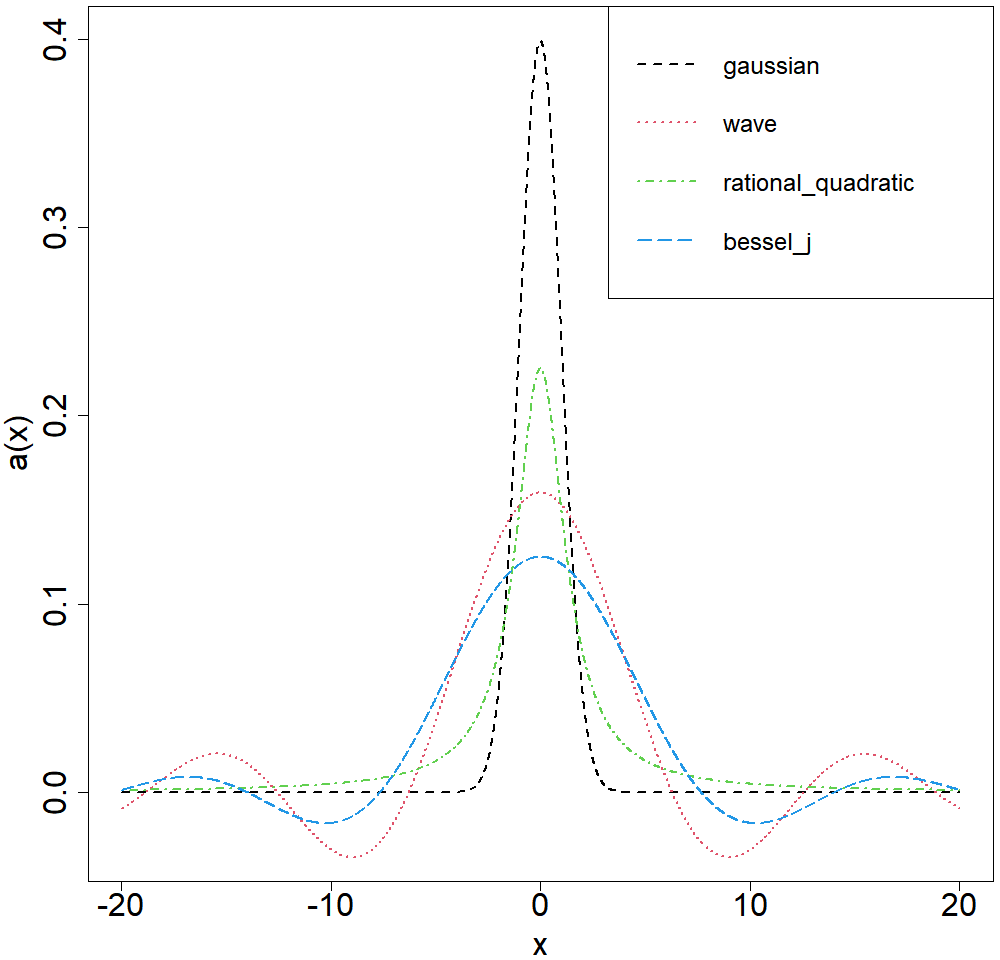
\includegraphics[keepaspectratio]{figures/symmetric_kernels.png}}
\end{minipage}
\caption{Examples of main available symmetric kernels where
\(\theta = 2, \nu = d = \alpha = \beta = 1 .\)}\label{fig:kernels_symm}
\end{figure}

\begin{figure}[!htb]
\centering
\begin{minipage}[t]{0.225\linewidth}
\centering
\end{minipage}
\hfill
\begin{minipage}[t]{0.225\linewidth}
\centering

\pandocbounded{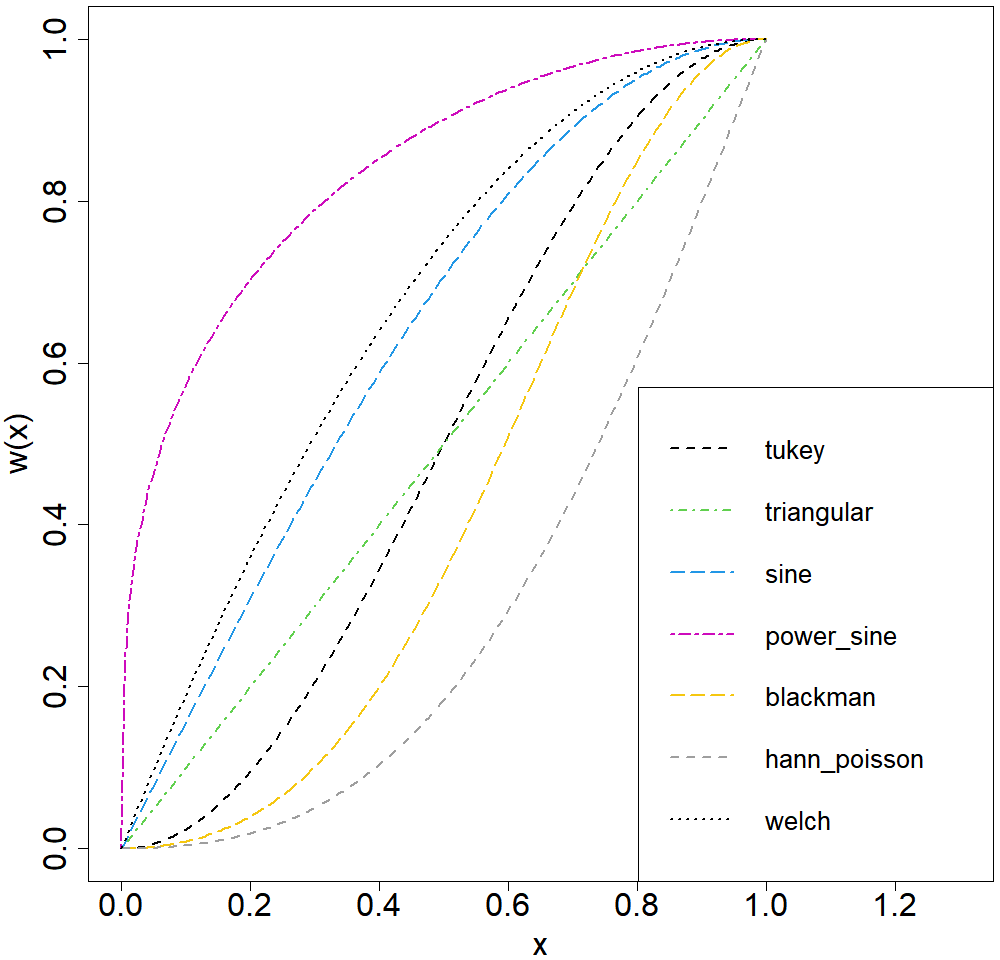
\includegraphics[keepaspectratio]{figures/windows.png}}
\end{minipage}
\hfill
\begin{minipage}[t]{0.225\linewidth}
\hfill
\end{minipage}
\hfill
\begin{minipage}[t]{0.225\linewidth}
\centering

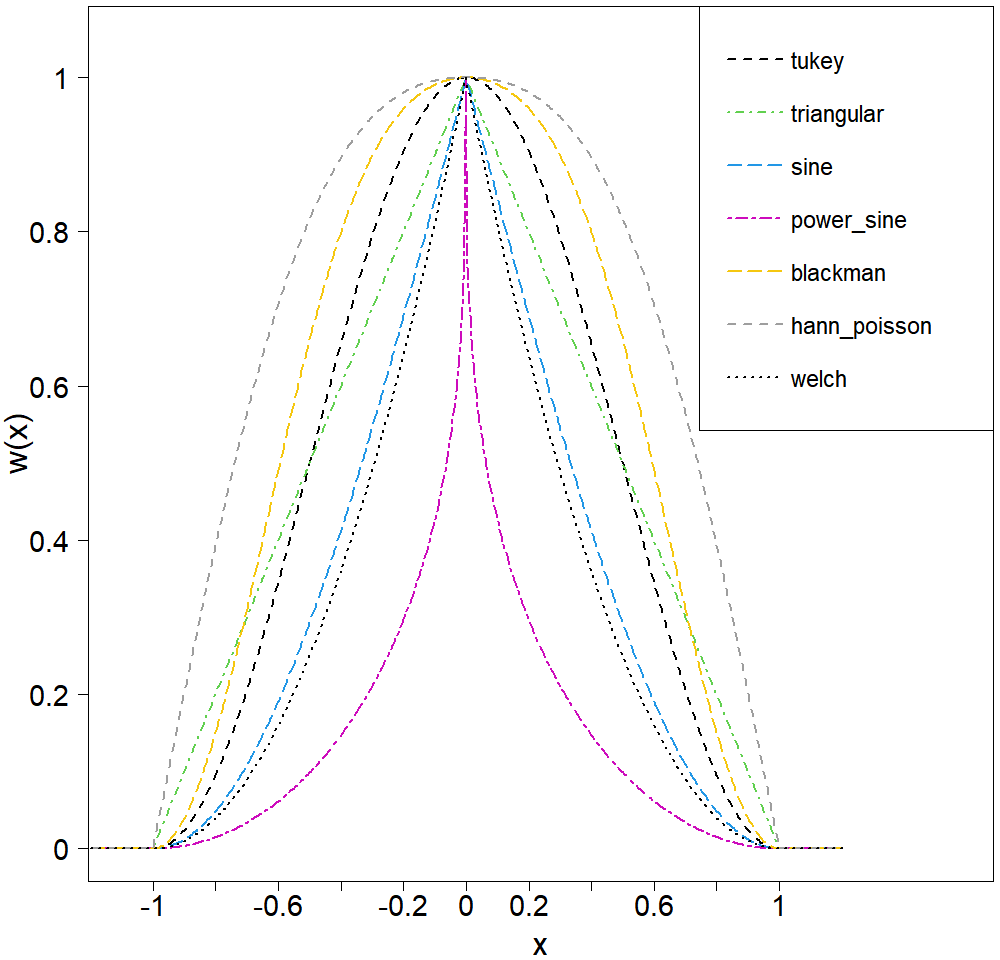
\includegraphics[width=1\linewidth,height=\textheight,keepaspectratio]{figures/windows_symm.png}
\end{minipage}
\caption{Examples of main available symmetric window functions where
\(a = 0.3, 0.16, 1\) for the power sine, Blackman and Hann-Poisson
window functions, respectively.}\label{fig:windows_symm}
\end{figure}

\subsection{Example 1}\label{sec:example_1}

To illustrate the application of the estimators and their accuracy, we
will consider a simulated Gaussian time series on a uniform grid on
\([0, 40]\) with a spacing of \(0.02,\) having a short-range dependent
Gaussian autocovariance model, \(\exp(-x^2)\). We will only estimate the
autocovariance function to a lag of 5, to use the recommended 10-20\% of
total samples \citep[Section~3.17]{Yaglom1987}.

The realisations were generated using the approach based on
eigendecomposition of the autocovariance matrix. Below is the code to
simulate the process and obtain the estimates based on the realisation
in Figure~\ref{fig:gaussian_realisation}, which are then plotted in
Figure~\ref{fig:gaussian}.

\begin{verbatim}
set.seed(135)
N <- 2001
x <- seq(0, 40, length.out = N)
Z <- rnorm(N)
dist_mat <- abs(outer(x, x, '-'))
cov_mat <- exp(- (dist_mat^2))
eig <- eigen(cov_mat)
X <- as.vector((eig$vectors %*% sqrt(diag(zapsmall(eig$values)))) %*% Z)

maxLag <- 251
t <- x[1:maxLag]

# standard estimators
Cs <- standard_est(X, maxLag = maxLag - 1, pd = FALSE, x = x)
Css <- standard_est(X, maxLag = maxLag - 1, pd = TRUE, x = x,
        type = "autocorrelation")

# Hall's estimators
hall_1 <- adjusted_est(X, x, t, 0.1, "gaussian", type = "autocorrelation")
hall_2 <- truncated_est(X, x, t, 3, 4, 0.1, "gaussian", type = "autocorrelation")

# tapered
tapered <- tapered_est(X, 1, "tukey", maxLag = maxLag - 1, x = x,
        type = "autocorrelation")

# splines
splines <- splines_est(X, x, Cs, 3, 2, maxLag = maxLag - 1, type = "autocorrelation")
Cs <- normalise_acf(Cs)

# Correction
corrected <- corrected_est(X, "gaussian", N_T=5*length(X), maxLag = maxLag - 1, x = x,
        type = "autocorrelation")

# Plot
par(mar=c(4,5.25,0.25,0.25)+.1)
plot(x[1:maxLag], exp(-x[1:maxLag]^2), type='l', lwd=2, ylim=c(-0.3, 1),
        xlab=expression(h), ylab=expression(hat(rho)*'(h)'), cex.axis=2,
        cex.lab=2)
lines(Cs, lwd=3, lty=2, col=2)
lines(Css, lwd=3, lty=3, col=3)
lines(hall_1, lwd=3, lty=4, col=4)
lines(hall_2, lwd=3, lty=5, col=6)
lines(tapered, lwd=3, lty=6, col=7)
lines(splines, lwd=3, lty=7, col=8)
lines(corrected, lwd=3, lty=8, col=13)

legend('topright', c('True', expression(hat('C')^'*'*'(h)'),
        expression(hat('C')^'**'*'(h)'), expression(hat('C')[H]*'(h)'),
        expression(hat('C')[1]*'(h)'), expression(hat('C')[N]^'a'*'(h)'),
        expression(hat('C')^'B'*('h')), expression('C'[T]^'(a)'*'(h)')),
        col=c(1, 2, 3, 4, 6, 7, 8, 13), lty=c(1, 2, 3, 4, 5, 6, 7, 8),
        lwd=c(2, rep(3, 7)), y.intersp=1, cex=2, ncol = 2)
\end{verbatim}

\begin{figure}[!tbp]
\centering
\begin{minipage}[t]{0.3\linewidth}
\centering

\pandocbounded{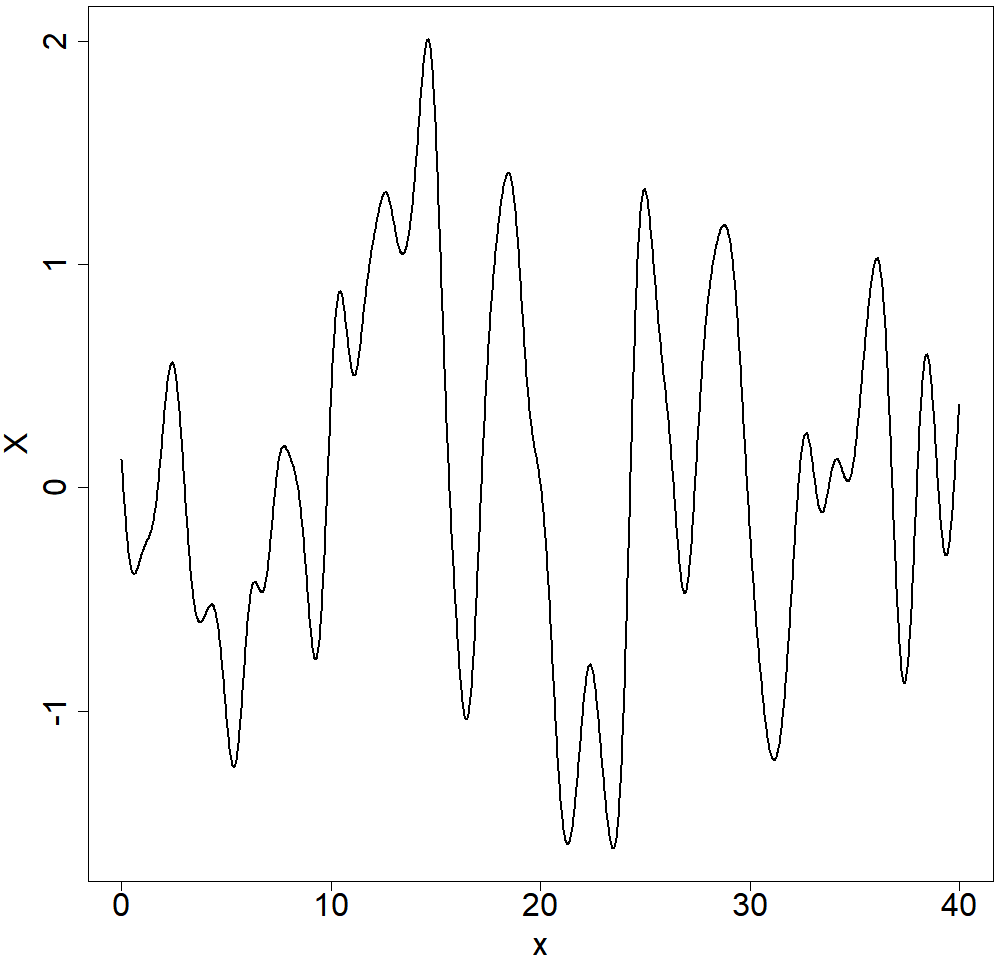
\includegraphics[keepaspectratio]{figures/gaussian_realisation.png}}
\end{minipage}
\hfill
\begin{minipage}[t]{0.3\linewidth}
\hfill
\end{minipage}
\hfill
\begin{minipage}[t]{0.3\linewidth}
\centering

\pandocbounded{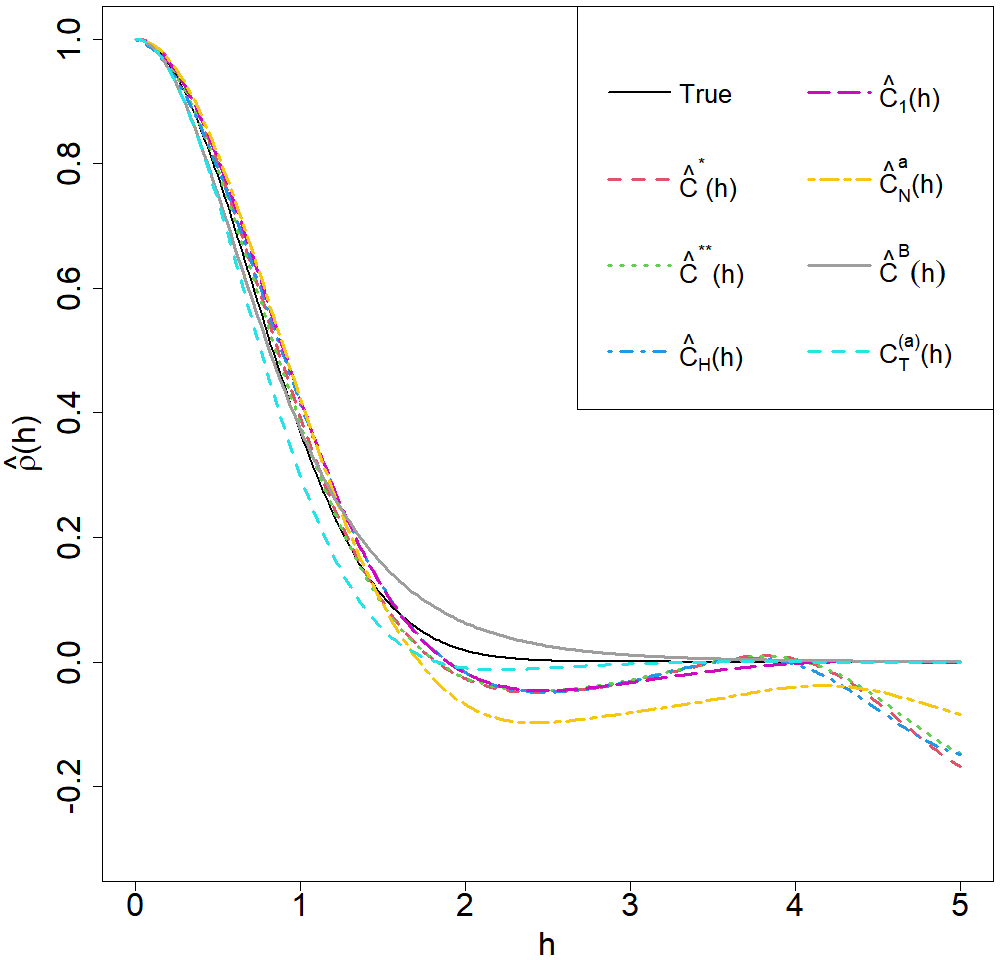
\includegraphics[keepaspectratio]{figures/gaussian.png}}
\end{minipage}
\caption{Estimated autocorrelation functions for a short-range dependent
time series.}\label{fig:gaussian}
\end{figure}

Whilst for short distances, the majority of the estimated
autocorrelation functions are consistent and adequately reflect the true
autocorrelation function, it is clear that for increasing distances the
waves start to overwhelm the estimators, seen in
Figure~\ref{fig:gaussian}. The waves are eliminated when applying the
estimators \(\widehat{C}_{1}(h)\) and \(C_{T}^{(a)}(h),\) given by
\eqref{eq:hall_trunc} and \eqref{eqn:kernel_correction_std_pd},
respectively.

For this and the following examples, we consider the estimated
autocorrelation functions instead of the estimated autocovariance
functions to allow for easier comparison.

Figure~\ref{fig:hall_area} plots the area (in grey) between estimators
given by~\eqref{eq:hall_est} (red) and \eqref{eq:hall_trunc} (green). As
the green curve is forced to zero after \(h=4,\) the area between the
two estimates increases after that point. The estimated area between
them is approximately 0.061. This difference can also be seen in the
plot of distances between the two estimates in
Figure~\ref{fig:hall_dist}. For \(h < 3,\) the estimates are rather
close. However, the distance starts to increase after this point
dramatically. The maximum distance between the two estimates is 0.1.
These values and plots can be produced as follows:

\begin{verbatim}
area_between(hall_1, hall_2, plot=T)
max_distance(hall_1, hall_2, plot=T)
\end{verbatim}

\begin{figure}[!htb]
\centering
\begin{minipage}[t]{0.3\linewidth}
\centering

\pandocbounded{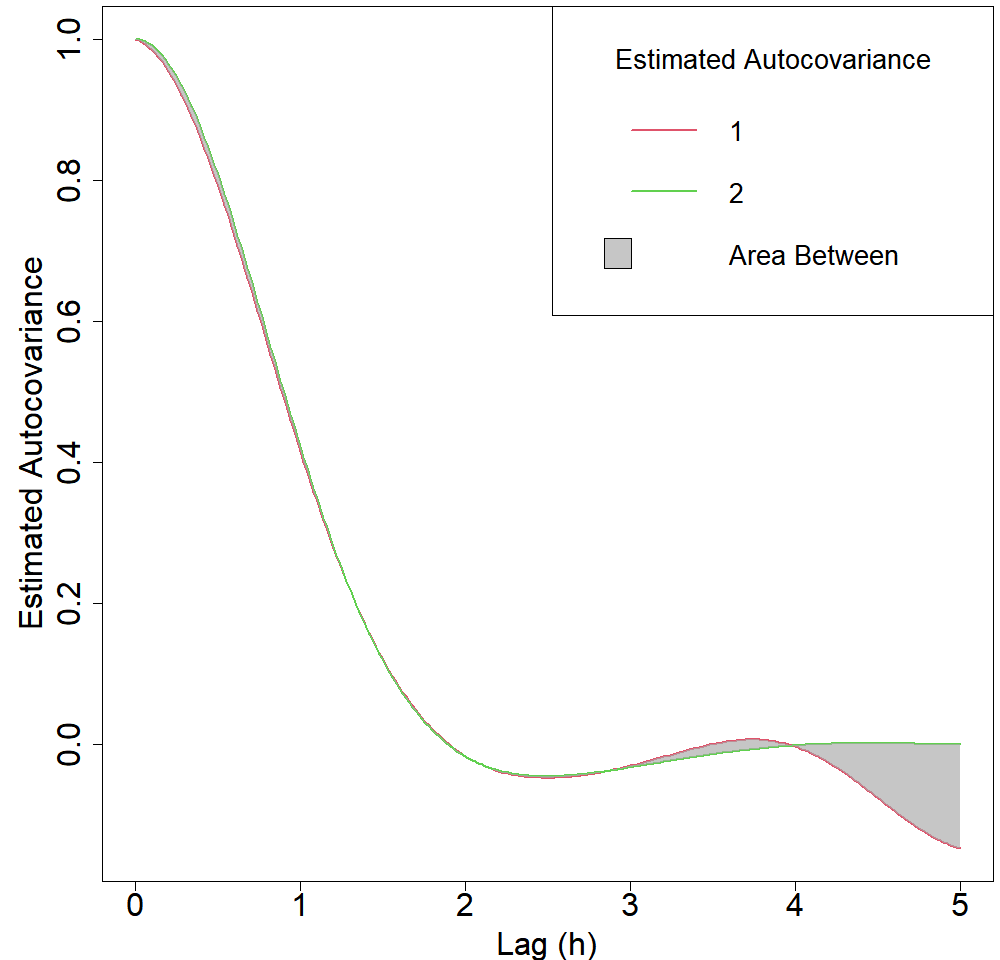
\includegraphics[keepaspectratio]{figures/hall_area_2.png}}
\end{minipage}
\hfill
\begin{minipage}[t]{0.3\linewidth}
\hfill
\end{minipage}
\hfill
\begin{minipage}[t]{0.3\linewidth}
\centering

\pandocbounded{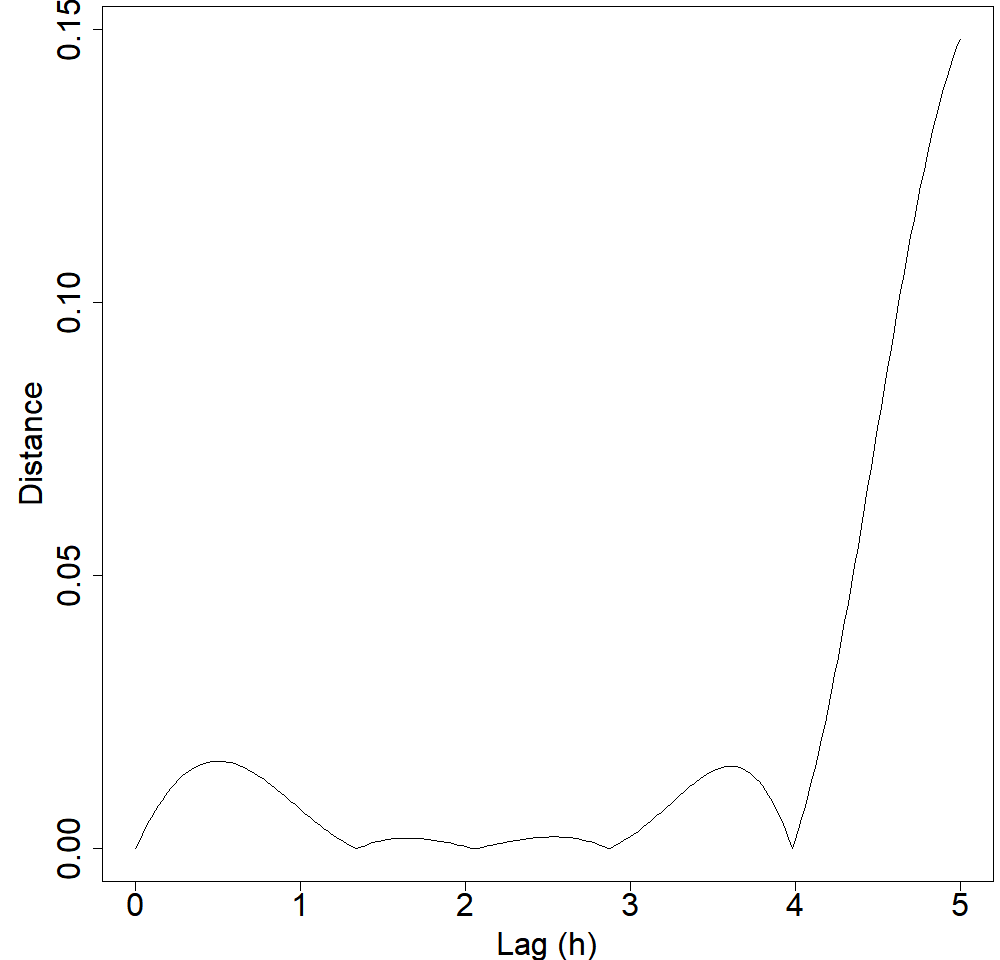
\includegraphics[keepaspectratio]{figures/hall_dist_2.png}}
\end{minipage}
\caption{Distances between estimated autocovariance
functions.}\label{fig:hall_dist}
\end{figure}

To compute the moving block and circular bootstrap for
estimator~\eqref{eq:std_est_pd}, one can use the following commands

\begin{verbatim}
plot(block_bootstrap(X, maxLag, x, l = maxLag), ylim=c(-0.25, 1), cex.axis=2, cex.lab=2)
plot(block_bootstrap(X, maxLag, x, l = maxLag, boot_type = 'circular'),
        ylim=c(-0.25, 1), cex.axis=2, cex.lab=2)
\end{verbatim}

Figures~\ref{fig:moving_boot} and \ref{fig:circular_boot} show graphical
outputs from the \code{block\_boostrap} function, where the
autocovariance functions are plotted. The solid black line is the
estimated autocovariance function, the red dashed line is the average
bootstrap autocovariance function, and the grey shaded bootstrap 95\%
confidence region is calculated pointwise for each lag. Both bootstrap
estimates give similar results, with the bootstrap estimate lessening
constant summation effects, compared to the original estimate that dips
after lag 4.

\begin{figure}[!htb]
\centering
\begin{minipage}[t]{0.3\linewidth}
\centering

\pandocbounded{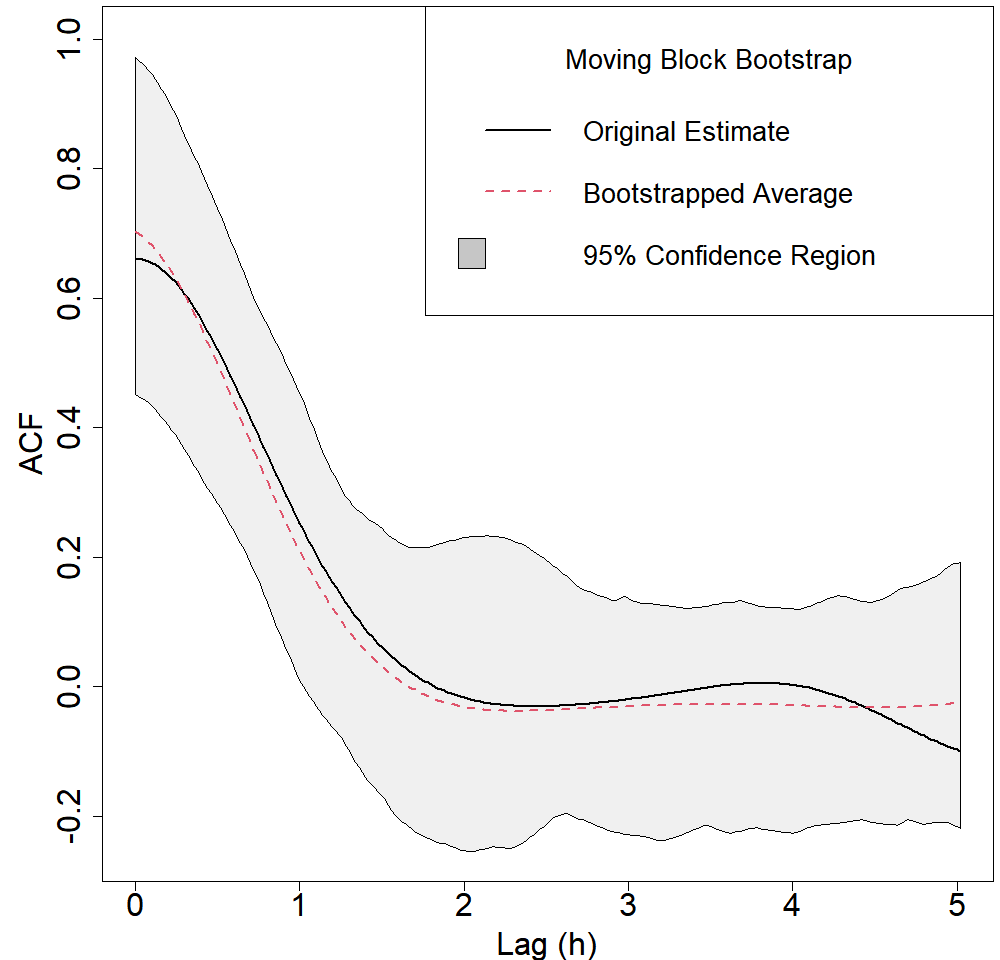
\includegraphics[keepaspectratio]{figures/moving_bootstrap.png}}
\end{minipage}
\hfill
\begin{minipage}[t]{0.3\linewidth}
\hfill
\end{minipage}
\hfill
\begin{minipage}[t]{0.3\linewidth}
\centering

\pandocbounded{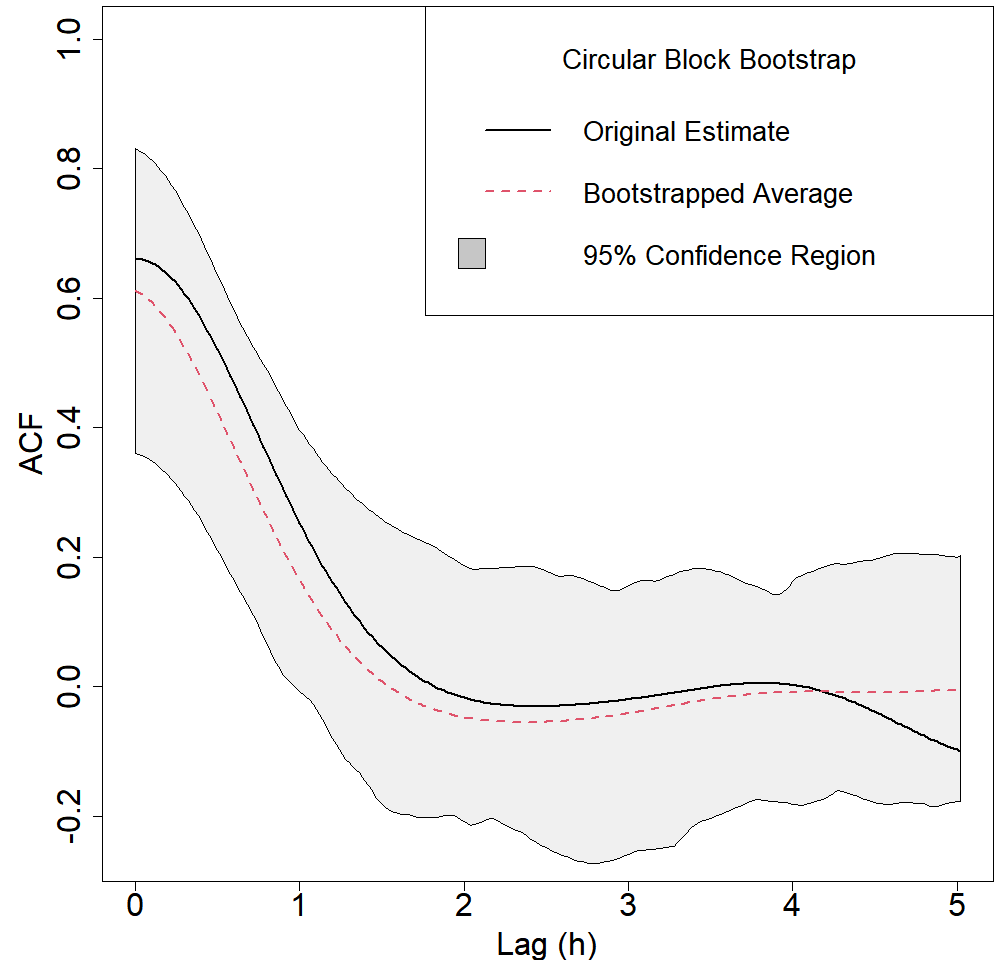
\includegraphics[keepaspectratio]{figures/circular_bootstrap.png}}
\end{minipage}
\caption{Circular block bootstrap estimates and confidence
region.}\label{fig:circular_boot}
\end{figure}

\subsection{Example 2}\label{example-2}

This example uses the classical yearly sunspot count data from 1700 to
1988, \texttt{sunspot.year}, available in the \pkg{datasets} R package.
This data gives the number of observed yearly sunspots, seen in
Figure~\ref{fig:sunspots_data}. It has been shown that the number of
sunspots exhibits long-range dependent and cyclic behaviours, see
\citet{GilAlana2009} and \citet{Hu2009}, with an approximate 11-year
cycle. So, one should expect to see periodicity in the autocovariance
estimate at multiples of lag 11. The example demonstrates that
estimator~\eqref{eq:hall_trunc} has potential issues as its Fourier
transform at the corresponding second nonzero frequency takes a negative
value. So, only one nonzero frequency can be used to obtain the
corrected estimates. Thus, this positive-definite adjustment will not
produce any useful result and is not reported. Instead, it is replaced
with the non-positive-definite version of estimator~\eqref{eq:hall_est},
denoted by \(\widehat{C}_{H}^{1}(h)\) in the legend of
Figure~\ref{fig:sunspots}. The splines estimator will also be omitted as
it does not capture the cyclicality in the autocovariance function.

\begin{figure}[!htb]
\centering
\begin{minipage}[t]{0.18\linewidth}
\centering
\end{minipage}
\hfill
\begin{minipage}[t]{0.18\linewidth}
\centering

\pandocbounded{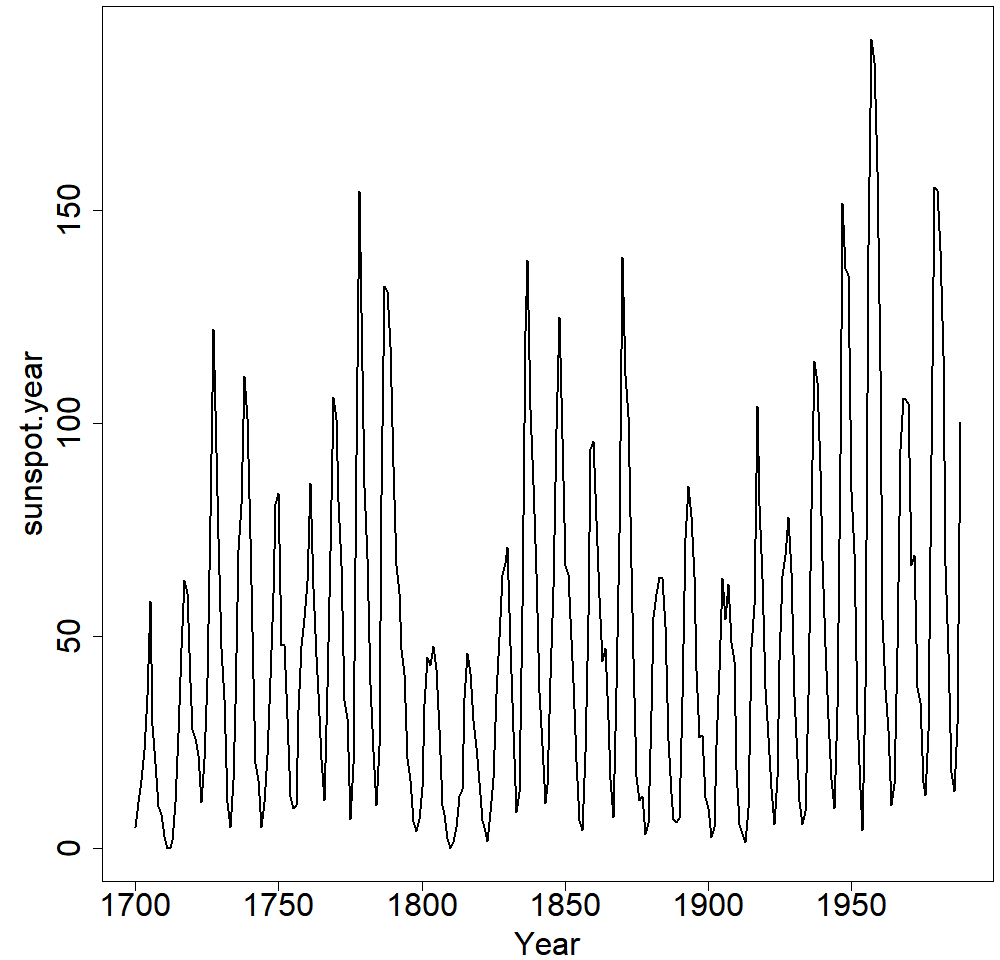
\includegraphics[keepaspectratio]{figures/sunspot_year.png}}
\end{minipage}
\hfill
\begin{minipage}[t]{0.18\linewidth}
\hfill
\end{minipage}
\hfill
\begin{minipage}[t]{0.18\linewidth}
\centering
\end{minipage}
\hfill
\begin{minipage}[t]{0.18\linewidth}
\centering

\pandocbounded{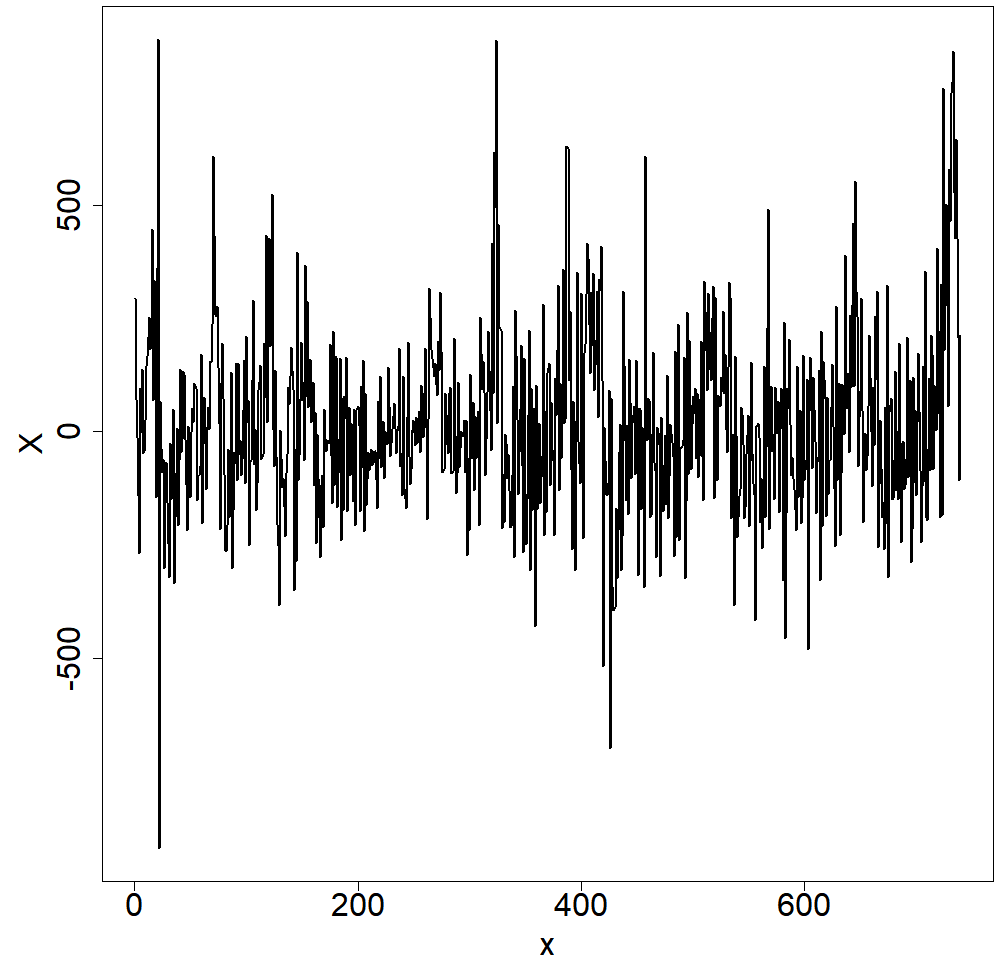
\includegraphics[keepaspectratio]{figures/bls_series.png}}
\end{minipage}
\caption{Increments of US unemployment count
data.}\label{fig:bls_series}
\end{figure}

\begin{figure}[!htb]
\centering
\begin{minipage}[t]{0.18\linewidth}
\centering    
\end{minipage}
\hfill
\begin{minipage}[t]{0.18\linewidth}
\centering

\pandocbounded{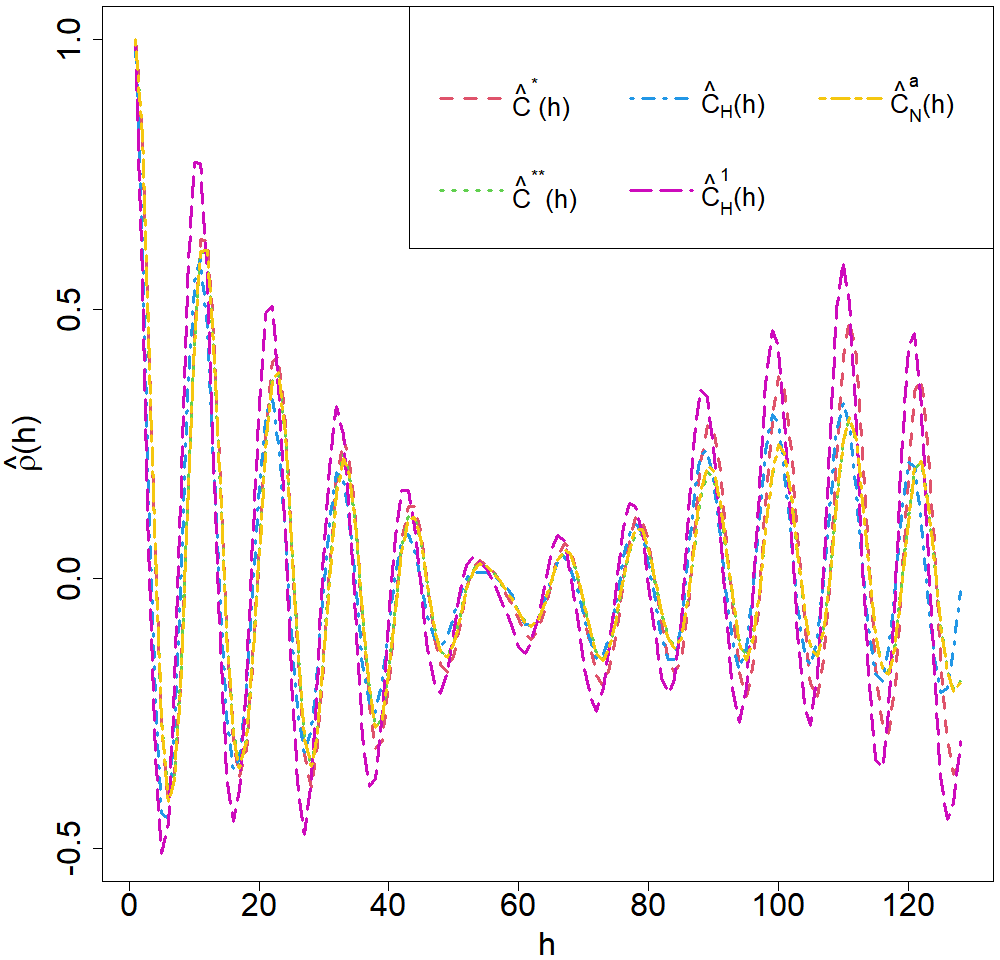
\includegraphics[keepaspectratio]{figures/sunspots.png}}
\end{minipage}
\hfill
\begin{minipage}[t]{0.18\linewidth}
\hfill
\end{minipage}
\hfill
\begin{minipage}[t]{0.18\linewidth}
\centering
\end{minipage}
\hfill
\begin{minipage}[t]{0.18\linewidth}
\centering

\pandocbounded{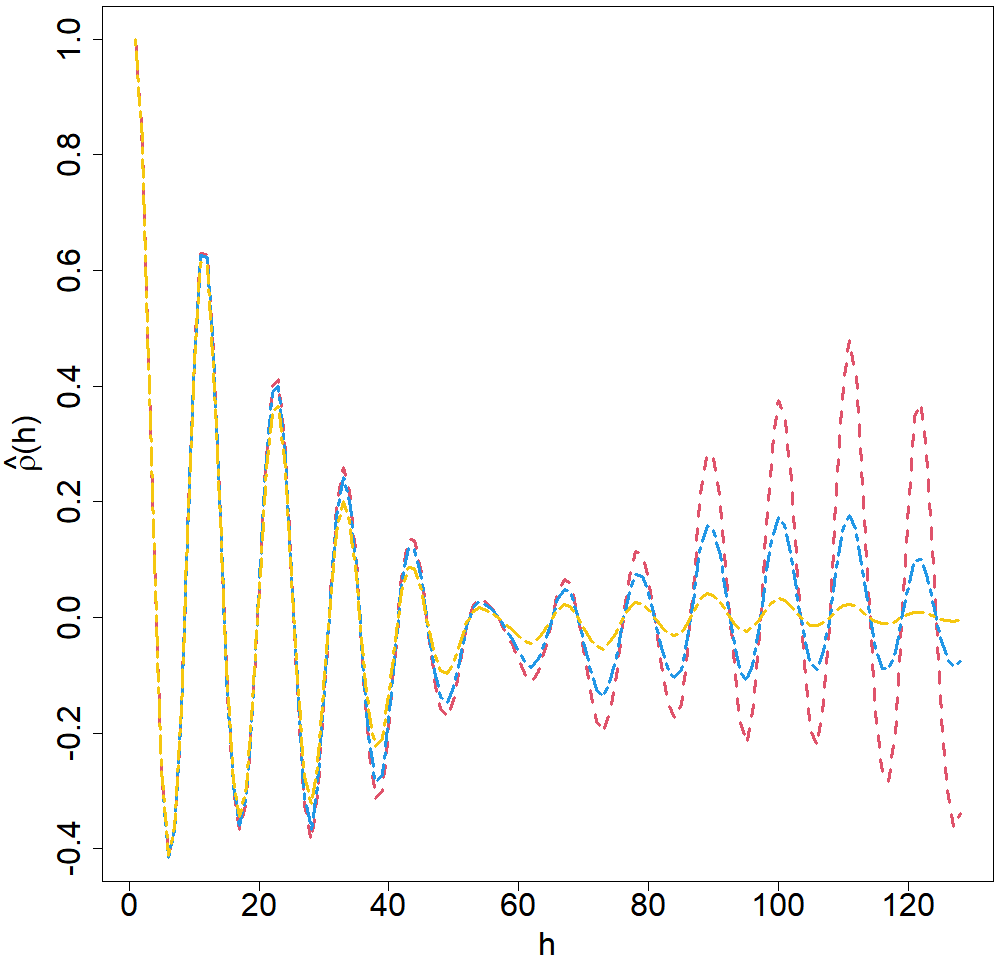
\includegraphics[keepaspectratio]{figures/sunspot_smoothed.png}}
\end{minipage}
\caption{Smoothing of \(C^{*}(h)\) autocorrelation
estimate.}\label{fig:smooth_sunspot}
\end{figure}

\begin{verbatim}
X <- as.vector(sunspot.year)
x <- 1:length(X)
maxLag <- 128

# standard estimators
Cs <- standard_est(X, maxLag = maxLag - 1, pd = FALSE, meanX = mean(X), x = x,
        type = "autocorrelation")
Css <- standard_est(X, maxLag = maxLag - 1, pd = TRUE, meanX = mean(X), x = x,
        type = "autocorrelation")

# Hall's estimators
hall_1 <- adjusted_est(X, x, x[1:maxLag], b = 0.1, kernel_name = "wave",
        type = "autocorrelation")
hall_2 <- adjusted_est(X, x, x[1:maxLag], b = 0.1, kernel_name = "wave", pd = FALSE,
        type = "autocorrelation")

# tapered
tapered <- tapered_est(X, 0.01, "tukey", maxLag = maxLag - 1, x = x,
        type = "autocorrelation")

par(mar=c(4,5.25,0.25,0.25)+.1)

plot(Cs, lwd=3, lty=2, col=2, type='l', ylim=c(-0.5, 1), xlab=expression(h),
        ylab=expression(hat(rho)*'(h)'), cex.axis=2, cex.lab=2)
lines(Css, lwd=3, lty=3, col=3)
lines(hall_1, lwd=3, lty=4, col=4)
lines(hall_2, lwd=3, lty=5, col=6)
lines(tapered, lwd=3, lty=6, col=7)

legend('topright', c(expression(hat('C')^'*'*'(h)'), expression(hat('C')^'**'*'(h)'),
        expression(hat('C')[H]*'(h)'), expression(hat('C')[H]^'1'*'(h)'),
        expression(hat('C')[N]^'a'*'(h)')), col=c(2, 3, 4, 6, 7),
        lty=c(2, 3, 4, 5, 6), lwd=c(rep(3, 5)), y.intersp=1, cex=1.7, ncol=3)
\end{verbatim}

As shown in Figure~\ref{fig:sunspots}, the estimators provide consistent
results. However, since no seasonal adjustment or transformation was
applied, the estimates may not correspond to the optimal model
specification for these data.

We have provided an example of how waves can be reduced and eliminated
from the estimates in Figure~\ref{fig:smooth_sunspot}. The red line, the
original estimate (computed using estimator~\eqref{eq:std_est}), behaves
cyclically and has waves of larger amplitude as the estimation lag
increases. The blue and yellow lines show the smoothing results by using
the wave (with \(\theta = 50)\)) and Gaussian (with \(\theta = 4000\))
kernels, respectively. Such kernels were chosen to lessen constant
summation and other unwanted effects and to bring the estimator to zero.
The latter correction may be appropriate when short-range dependence is
expected.

\subsection{Example 3}\label{example-3}

We use monthly changes in U.S. unemployment counts data studied by
\citet{Artiach2011} and sourced from the U.S. Bureau of Labor Statistics
\url{https://www.bls.gov/}. There are 739 months of observations in the
time series plotted in Figure~\ref{fig:bls_series}. We estimated the
autocovariance function up to a lag of 144, representing a maximum
difference of 12 years between observations. In \cite{Artiach2011}, the
periodogram of this time series has a nonzero singularity indicating
cyclic long-memory, see~\cite{Olenko2022}, where each cycle is roughly
5.5 years. So, we should expect some cyclicality in the estimated
autocovariance functions.

\begin{figure}[!htb]
\centering
\begin{minipage}[t]{0.225\linewidth}
\centering
\end{minipage}
\hfill
\begin{minipage}[t]{0.225\linewidth}
\centering

\pandocbounded{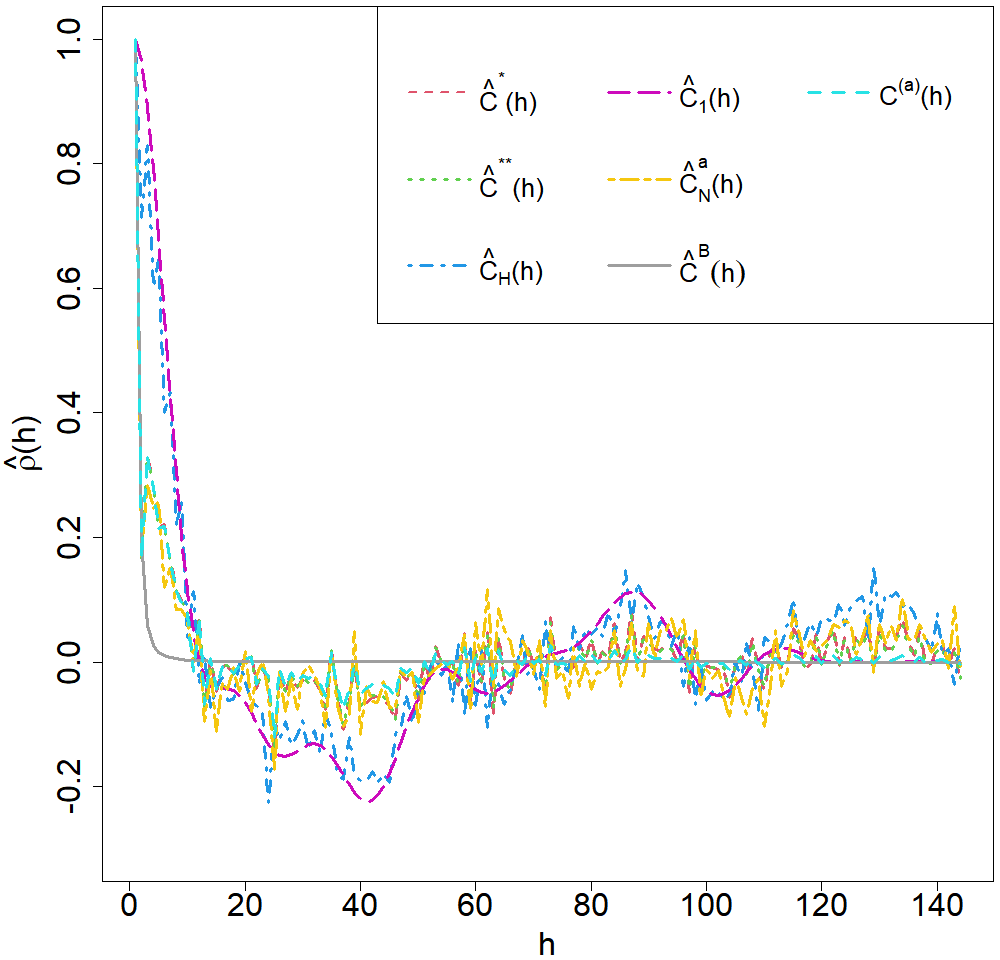
\includegraphics[keepaspectratio]{figures/bls.png}}
\end{minipage}
\hfill
\begin{minipage}[t]{0.225\linewidth}
\hfill
\end{minipage}
\hfill
\begin{minipage}[t]{0.225\linewidth}
\centering

\pandocbounded{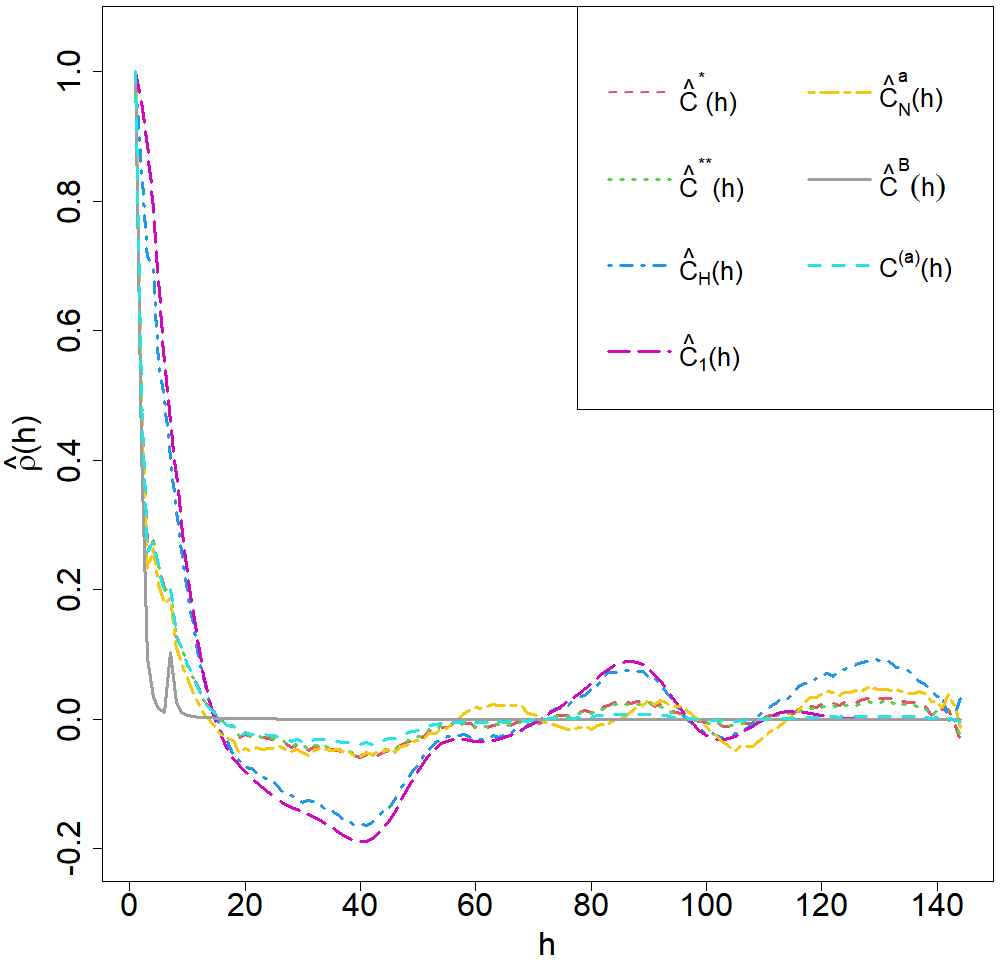
\includegraphics[keepaspectratio]{figures/bls_smooth2.png}}
\end{minipage}
\caption{Smoothing of estimates for the unemployment increments
data.}\label{fig:smooth_bls}
\end{figure}

The following code produces the estimated autocorrelations plotted in
Figure~\ref{fig:bls}.

\begin{verbatim}
maxLag <- 144
X <- X_bls
x <- 1:length(X)

# standard estimators
Cs <- standard_est(X, maxLag = maxLag - 1, pd = FALSE, x = x)
Css <- standard_est(X, maxLag = maxLag - 1, pd = TRUE, x = x,
        type = "autocorrelation")

# Hall's estimators
hall_1 <- adjusted_est(X, x, x[1:maxLag], b = 0.1, kernel_name = "rational_quadratic",
        type = "autocorrelation")
hall_2 <- truncated_est(X, x, x[1:maxLag], 110, 120, b = 0.1,
        kernel_name = "rational_quadratic", type = "autocorrelation")

# tapered
tapered <- tapered_est(X, 1, "tukey", maxLag = maxLag - 1, x = x,
        type = "autocorrelation")

# splines
splines <- splines_est(X, x, Cs, 3, 2, maxLag = maxLag - 1, type = "autocorrelation")
Cs <- normalise_acf(Cs)

# Correction
corrected <- corrected_est(X, "rational_quadratic", N_T = 5*length(X), maxLag = maxLag - 1,
        x = x, type = "autocorrelation")

colours <- c(2, 3, 4, 6, 7, 8, 13)
ltys <- c(2, 3, 4, 5, 6, 7, 8)
par(mar=c(4,5.25,0.25,0.25)+.1)
plot(Cs, lwd=3, lty=2, col=2, type='l', ylim=c(-0.3, 1), xlab=expression(h),
        ylab=expression(hat(rho)*'(h)'), cex.axis=2, cex.lab=2)
lines(Css, lwd=3, lty=3, col=3)
lines(hall_1, lwd=3, lty=4, col=4)
lines(hall_2, lwd=3, lty=5, col=6)
lines(tapered, lwd=3, lty=6, col=7)
lines(splines, lwd=3, lty=7, col=8)
lines(corrected, lwd=3, lty=8, col=13)

legend('topright', c(expression(hat('C')^'*'*'(h)'), expression(hat('C')^'**'*'(h)'),
        expression(hat('C')[H]*'(h)'), expression(hat('C')[1]*'(h)'),
        expression(hat('C')[N]^'a'*'(h)'), expression(hat('C')^'B'*('h')),
        expression('C'^'(a)'*'(h)')), col=colours, lty=ltys, lwd=c(2, rep(3, 6)),
        y.intersp=1.2, cex=1.8, ncol=3)
\end{verbatim}

As can be seen from Figure~\ref{fig:bls}, the estimates have local
chaotic fluctuations. To better see the main pattern of the estimates,
Figure~\ref{fig:smooth_bls} shows the application of a moving average to
each of the estimators in Figure~\ref{fig:bls}. After this smoothing,
two estimators, \eqref{eq:hall_est} and \eqref{eq:hall_trunc}, exhibit
cyclicality expected for this data.

\subsection{Example 4}\label{example-4}

This example empirically investigates the computational complexity of
the methods by evaluating the runtime and memory usage of the
estimators. Autocovariance function estimates were computed for a
sequence of simulated time series with Gaussian autocovariance, similar
to \hyperref[sec:example_1]{Example 1}. The realisations of the time
series were simulated on uniform grids over \([0, 40]\) with lengths
\(N=101, 151, \dots, 951, 1001\). This process was repeated 100 times,
and the results presented are the medians.

Figure~\ref{fig:time_all} shows the log10-time of the computed
estimators. The log scale was used due to the large difference between
estimators. For example, estimator~\eqref{eq:std_est_pd} was computed in
0.000781015 seconds, on average, for a time series of length
\(N = 1001,\) whilst estimator~\eqref{eq:hall_est} was computed in
8.45674 seconds. It is clear that all estimators~\eqref{eq:std_est},
\eqref{eq:std_est_pd}, \eqref{eq:tapered_est}, and
\eqref{eqn:kernel_correction_std_pd} perform similarly in terms of time,
whilst Hall's estimators~\eqref{eq:hall_est} and \eqref{eq:hall_trunc}
exhibit significant growth in computational time. The splines
estimator~\eqref{eq:splines_est} shows a consistent time usage across
all estimates, exhibiting minimal growth as \(N\) increases.

\begin{figure}[!htbp]
\centering
\begin{minipage}[t]{0.225\linewidth}
\centering
\end{minipage}
\hfill
\begin{minipage}[t]{0.225\linewidth}
\centering

\pandocbounded{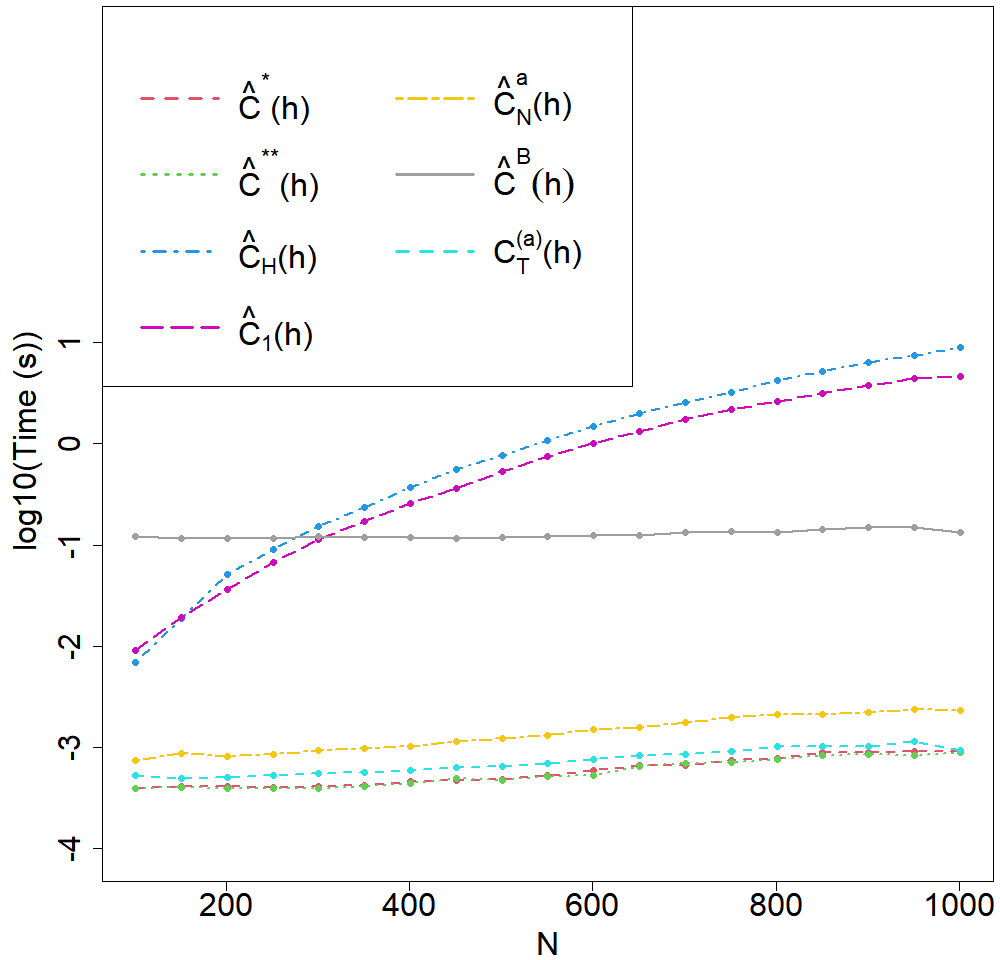
\includegraphics[keepaspectratio]{figures/log_time_all_100_iters.png}}
\end{minipage}
\hfill
\begin{minipage}[t]{0.225\linewidth}
\hfill
\end{minipage}
\hfill
\begin{minipage}[t]{0.225\linewidth}
\centering

\pandocbounded{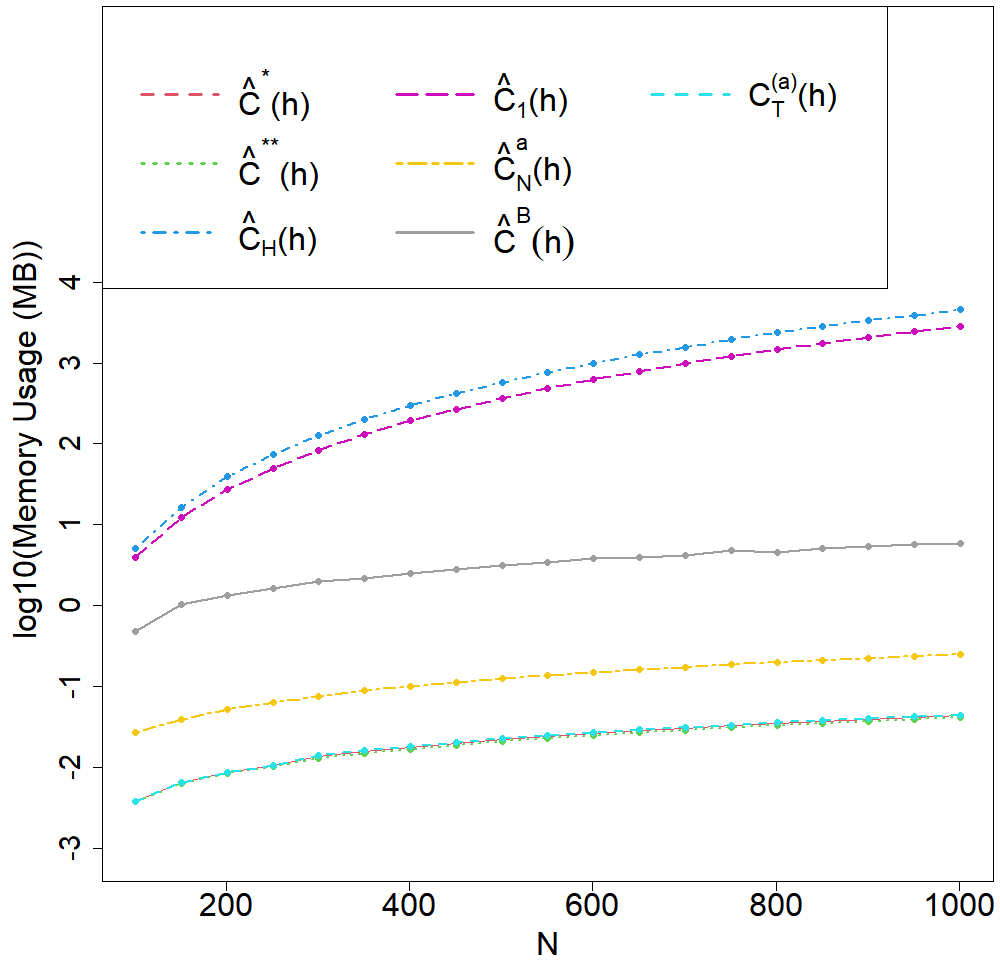
\includegraphics[keepaspectratio]{figures/log_memory_all_100_iters.png}}
\end{minipage}
\caption{Log-scale memory usage (MB) for estimates for time series of
varying length.}\label{fig:memory_all}
\end{figure}

Figure~\ref{fig:memory_all} shows the log10-memory usage, where the
log-scale was chosen for the same reasons as the time case. The
estimators~\eqref{eq:std_est}, \eqref{eq:std_est_pd}, and
\eqref{eqn:kernel_correction_std_pd} all effectively used the same
memory. The estimator~\eqref{eq:tapered_est} is quite close,
particularly in terms of growth; however, it is shifted upward. Again,
Hall's estimators~\eqref{eq:hall_est} and \eqref{eq:hall_trunc} exhibit
significantly greater memory usage growth than the other estimators. The
splines estimator~\eqref{eq:splines_est} is stable in terms of growth,
as in the time case.

It is clear that Hall's estimators, \eqref{eq:hall_est} and
\eqref{eq:hall_trunc}, require significantly more computational time and
memory usage compared to other estimators. Thus, these estimators may
not be appropriate in the case of Big Data. The other estimators are
computed relatively quickly and require significantly less memory, even
for large values of \(N.\) Further, these limitations should be
considered when performing block bootstrap or other statistical
procedures involving repeated computation of estimated covariances
(e.g., moving window analysis, model diagnostics, Kriging/Gaussian
process prediction and interpolation), as the estimator must be called
many times. In such cases, using parallelism options, as implemented in
the package for bootstrap, may substantially reduce computational time.

\section{Summary}\label{summary}

The article introduced the package \CRANpkg{CovEsts}, which provides
several nonparametric autocovariance function estimators available in
the literature. The package offers a set of functions that allow users
to easily apply the different estimators, as shown in the examples. The
autocovariance estimator functions have a high level of flexibility with
various options that the user can control, such as a custom kernel,
selecting the sampling grid, and controlling the positive-definiteness
of estimators, among others. Several functions are provided to generate
bootstrap autocovariance confidence regions and to address potential
issues in autocovariance estimation. In addition, various metrics are
included to compare the performance of the estimators. In the future,
the package is planned to be extended to work with similar nonparametric
estimators for spatial data.

\section{Computation details}\label{computation-details}

R version 4.5 was used to develop, test the package, and produce all
outputs in this article.

\section{Acknowledgement}\label{acknowledgement}

This research was partially supported by the Australian Research Council
Discovery Projects funding scheme (project DP220101680). Andriy Olenko
was also partially supported by La Trobe University's SCEMS CaRE and
Beyond grant. The authors are grateful to Professors N. Cressie, N.
Leonenko, and E. Porcu for their feedback on certain approaches to the
nonparametric estimation of covariance functions. We also thank the
editor, Prof. R.~J.~Hyndman, and anonymous reviewers for their comments
that helped to improve the package and the paper.

% LaTeX author address
\address{Adam Bilchouris\\
Department of Mathematics and Statistics\\
La Trobe University\\
Australia\\
ORCiD: 0009-0002-4649-0247\\
\email{a.bilchouris@latrobe.edu.au}}
\address{Andriy Olenko\\
Department of Mathematics and Statistics\\
La Trobe University\\
Australia\\
ORCiD: 0000-0002-0917-7000\\
\email{a.olenko@latrobe.edu.au}}
% LaTeX bib file link
\bibliography{bilchouris-olenko.bib}
